%@def.tex
\documentclass[landscape]{slides}
\usepackage[warn]{mathtext}
\usepackage[T2A]{fontenc}
\usepackage[utf8]{inputenc}
\usepackage[english, russian]{babel}
\usepackage{indentfirst}
\usepackage{amsmath, amsfonts, amssymb}
\usepackage{geometry}
\usepackage{hyperref}
\usepackage{wrapfig}
\geometry{top=2cm}
\geometry{left=3cm}
\geometry{right=2cm}
\geometry{bottom=2cm}
\usepackage{color}
\usepackage{multirow}
\usepackage{lscape}
\usepackage{wrapfig}
\usepackage{graphicx}
\usepackage{epstopdf}
\usepackage{tikz}
\usepackage{tikz-3dplot}
\usetikzlibrary{arrows}
\usetikzlibrary{calc}

\renewcommand{\vec}{\overline}
\renewcommand{\phi}{\varphi}

\graphicspath{{pics/}}

\makeatletter
\newcommand{\nextverbatimspread}[1]{%
    \def\verbatim@font{%
        \linespread{#1}\normalfont\ttfamily% Updated definition
            \gdef\verbatim@font{\normalfont\ttfamily}}% Revert to old definition
}
\makeatother

\newenvironment{mintemize}{%
    \vspace{-1.5em}
    \begin{itemize}
        \setlength\itemsep{-0.2em}
}
{
    \end{itemize}
    \vspace{-1em}
}

\newenvironment{cslide}{%
    \begin{slide}
    \begin{center}
}
{
    \end{center}
    \end{slide}
}

\makeatletter
\def\sltop{\let\@topfil\relax}
\makeatother

\newenvironment{tslide}[1]{%
    \begin{slide}
    \sltop
    {\large\textbf{#1}}
}
{ \end{slide} }


\begin{document}

\begin{cslide}
    
\includegraphics[width=3cm]{mai.eps}

    \large\textbf{ Разработка алгоритмов управления
    массивом беспилотных летательных аппаратов
    с целью построения информационного поля
    участка местности}

    \vfill

    \begin{flushright}
    \small Выполнил студент гр. 07-608 Бутко О.А.

    \small Руководитель Жидков В.Н.
    \end{flushright}

    \vfill

    \small Москва, 2015
\end{cslide}

\begin{tslide}{Постановка задачи}

Создание алгоритма исследования местности,
формирования цифровой карты, а также поддержание
ее в актуальном состоянии, посредством МБПЛА,
включает следующие этапы:
\begin{itemize}
\item Формализация модели цифровой карты
\item Формирование требований к системе МБПЛА для решения задачи построения карты
\item Формализация модели МБПЛА
\item Разработка алгоритма обхода выпуклых препятствий
\item Разработка алгоритма обхода местности
\item Разработка схемы и программного комплекса имитационного моделирования для различных вариантов алгоритма обхода:
    \begin{itemize}
    \item распределение подгрупп юнитов по регионам карты
    \item поиск ближайшего неизведанного региона
    \item выбор случайной точки в пространстве карты
    \end{itemize}
\item Проведение имитационного моделирования, обобщение и анализ полученных результатов.
\end{itemize}

\end{tslide}

\begin{tslide}{Формализация модели цифровой карты}

    \begin{wrapfigure}{r}{.3\linewidth}
    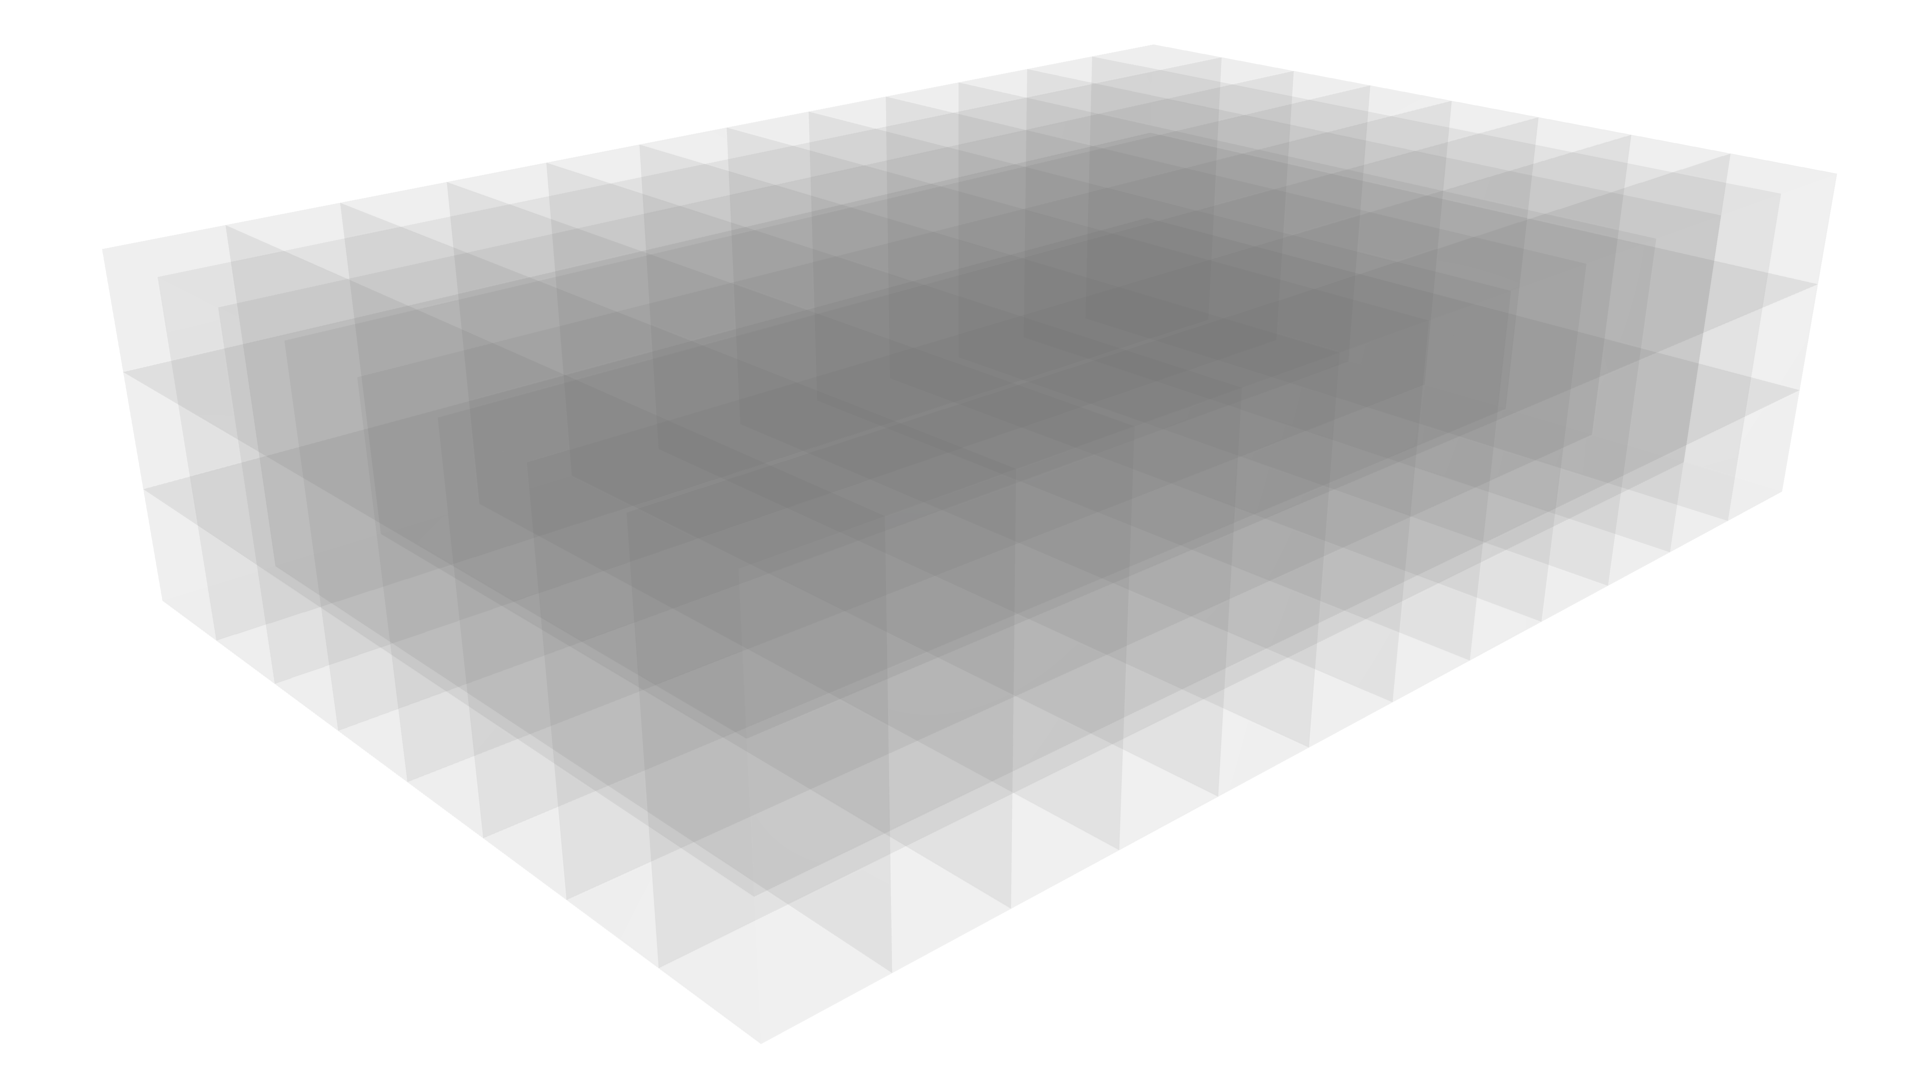
\includegraphics[width=\linewidth]{map.png}
    \vspace{-2cm}
    \end{wrapfigure}
    Ограничим участок исследуемой местности по высоте, ширине и глубине.
    Разобьём его на прямоугольные сектора, каждый из которых будет хранить
    информацию об единице объёма:
    \begin{itemize}
    \item \verb|N| -- количество проверок сектора
    \item \verb|T| -- последнее время проверки
    \item \verb|val| -- результат проверки (наличие объекта)
    \end{itemize}


    \begin{wrapfigure}{l}{.3\linewidth}
    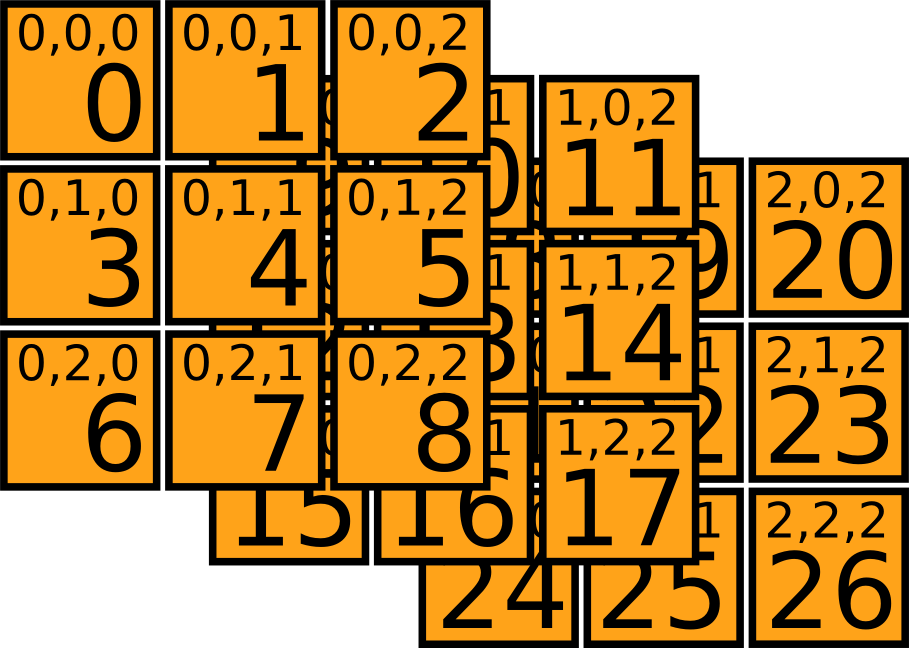
\includegraphics[width=\linewidth]{mapRealisation.png}
    \end{wrapfigure}

    Карта имеет матрицу трансформации для перевода из системы индексных
    координат в систему координат местности. Реализуем её в виде одномерного
    массива с возможностью 3х-мерной индексации.

    \begin{flushright}
    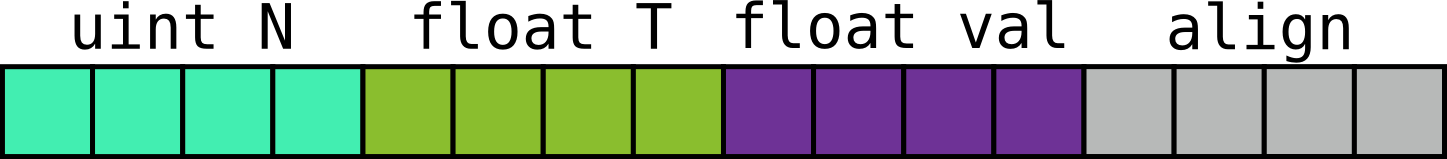
\includegraphics[width=\linewidth]{mapData.png}
    \end{flushright}

    Информация в секторе выровнена по 16 байтам.

\end{tslide}

\begin{tslide}{Формирование требований к системе МБПЛА для решения задачи построения карты}

    \begin{wrapfigure}{r}{0.3\textwidth}
        \vspace{-1cm}
        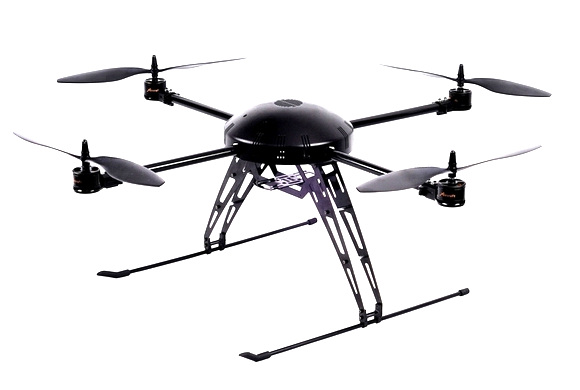
\includegraphics[width=\linewidth]{X650.jpg}
        \vspace{-3cm}
    \end{wrapfigure}

    За основу была взята концепция сверхлёгкого, малогабаритного БПЛА
    с вертикальным взлётом.

    Минимальные требования к системе МБПЛА,
    необходимые для решения поставленной задачи:
    \begin{itemize}
    \item количество юнитов может исчисляться\newline сотнями и тысячами
    \item каждый юнит знает свой фазовый вектор
    \item каждый юнит может запросить фазовые вектора остальных юнитов системы
    \item на борту юнита установлена поворотная камера,
        позволяющая получать информацию о дальности до объектов в каждом пикселе (карта глубин)

    \item у каждого юнита есть возможность запрашивать и изменять карту местности
    \end{itemize}

\end{tslide}

\begin{tslide}{Модель единицы массива}
    
    Модель БПЛА представляет из себя материальную точку,
    движущуюся под действием сил.

    Дифференциальное уравнение движения центра масс БПЛА:

    \begin{wrapfigure}{l}{.3\linewidth}
    $$
    \left\{
        \begin{array}{l l}
        \dot{\vec{X}}  & = \vec V \\
        \dot{\vec{V}}  & = \vec a + \vec g
        \end{array}
    \right.
    $$
    \vspace{-1cm}
    \end{wrapfigure}

    где: $\vec X, \vec V$ -- координаты и скорость юнита
    
    $\vec g$ -- ускорение свободного падения

    $\vec a = \frac{1}{m} \sum_{i=1}^N F_i$ -- ускорение от действующих на юнит сил

    Действующие на юнит силы

    \tikzstyle{every picture}+=[
        axis/.style={black},
        vector/.style={->,line width=1mm,black},
        help/.style={gray,thin,dashed},
        rot/.style={tdplot_rotated_coords}
    ]

    \def\sum{ circle[radius=2mm] }

    \tikzset{%
    block/.style    = {draw, thick, rectangle,
                        minimum height = 2em,
                        minimum width = 2em},
    input/.style    = {coordinate,circle,draw,scale=0.3,node distance=6cm}, % Input
    output/.style   = {coordinate}, % Output
    cross/.style={path picture={
                    \draw[black]
                (path picture bounding box.south east) -- (path picture bounding box.north west) (path picture bounding box.south west) -- (path picture bounding box.north east);
                }},
    sum/.style      = {draw,circle,cross} % Adder
    }

    \def\dot{circle[radius=1mm]}
    \def\P{1.9}
    \def\Pm{1.6}
    \def\Pmm{0.5}
    \def\Vrot{10}
    \def\fnlen{4}
    \def\ftlen{3}
    \def\dst{8}

    \begin{tabular}{l r}

    \tdplotsetmaincoords{0}{0}
    \begin{tikzpicture}[scale=0.6,tdplot_main_coords]
        \tdplotsetrotatedcoords{85}{60}{-50}

        \draw[rot,vector,blue] (0,0) -- (\dst,0);
        \node[rot,below right] at (6,0) {$\vec F_\text{упр}$};

        \draw[rot,vector] (0,0) -- (\Vrot:5) node[above] {$\vec V$};
        \draw[rot,vector,red] (0,0) -- (180+\Vrot:3);
        \node[rot,below] at (180+\Vrot:3) {$\vec F_\text{вс}$};
        \draw[rot,vector,green] (0,0) -- (-\fnlen,\ftlen,0);
        \node[rot,above left] at (-\fnlen,\ftlen) {$\vec F_{\text{кор}}$};

        \draw[rot,help] (-\fnlen,\ftlen) -- (\dst-\fnlen,\ftlen);
        \draw[rot,help] (\dst,0) -- (\dst-\fnlen,\ftlen);
        \draw[rot,help] (0,0) -- (\dst-\fnlen,\ftlen);
        \draw[rot,vector] (0,0) -- ($(\dst-\fnlen,\ftlen)+(180+\Vrot:3)$) node (S) {};
        \draw[rot,help] (180+\Vrot:3) -- (S);
        \draw[rot,help] (\dst-\fnlen,\ftlen) -- (S);

        \node[rot,left] at (S) {$\vec F$};
        \fill[rot,black] (0,0) \dot node[below] {$O$};

    \end{tikzpicture}

    &

    \begin{tikzpicture}[auto, thick, node distance=2cm, >=triangle 45,scale=1]
        \draw
        node[input] (input1) {} 
        node[sum, right of=input1] (suma1) {}
        node[input, below of=suma1] (input2) {} 
        node[block, right of=suma1] (PID) {$PID$};

        \draw[->] (input1) -- node[above left] {$\vec X$} (suma1);
        \draw[->] (input2) -- node[below left] {$\vec X_\text{цт}$} (suma1);
        \draw[->] (input2) -- node[above right] {$-$} (suma1);
        \draw[->] (suma1) -- node {} (PID);
        \draw[->] (PID) -- node[above right] {$\vec F_\text{упр}$} +(2cm,0);

    \end{tikzpicture}

    \end{tabular}

    \begin{itemize}

    \item $\vec F_\text{вс} = C_{x0}\frac{-\vec V \rho |V|}{2} S$ -- сила сопротивления воздуха
    \item $\vec F_\text{упр}$ -- управляющее воздействие (определяется положением целевой
    точки)
    \item $\vec F_\text{кор}$ -- коррекция по ближайшим опасным точкам
    \end{itemize}

\end{tslide}

\begin{tslide}{Алгоритм обхода препятствий}

    В целях предотвращения столкновений юнита с объектами был разработан
    алгоритм корекции управляющего воздействия по опасным точкам.
    К ближайшим опасным точкам относятся заполненные сектора карты и
    юниты системы.

    \tikzstyle{every picture}+=[
        axis/.style={black},
        vector/.style={->,line width=1mm,black},
        help/.style={gray,thin,dashed},
        rot/.style={tdplot_rotated_coords}
    ]

    \def\dot{circle[radius=1mm]}
    \def\P{1.9}
    \def\Pm{1.6}
    \def\Pmm{0.5}
    \def\Vrot{20}
    \def\fnlen{5}
    \def\ftlen{2}
    \def\dst{8}

    \begin{wrapfigure}{l}{.5\linewidth}
    \tdplotsetmaincoords{0}{0}
    \begin{tikzpicture}[scale=.8,tdplot_main_coords]
        \tdplotsetrotatedcoords{85}{60}{-50}
        \fill[rot,red] (\dst,  0,  0) \dot;
        \fill[rot,red] (\dst, .5,  0) \dot;
        \fill[rot,red] (\dst,-.5,  0) \dot;
        \fill[rot,red] (\dst, .5, .5) \dot;
        \fill[rot,red] (\dst,-.5, .5) \dot;
        \fill[rot,red] (\dst,  0, .5) \dot;
        \fill[rot,red] (\dst,  0,-.5) \dot;
        \fill[rot,red] (\dst, .5,-.5) \dot;
        \fill[rot,red] (\dst,-.5,-.5) \dot;

        \draw[rot,vector] (0,0,0) -- (\dst,0,0);
        \node[rot,above] at (6,0,0) {$\vec D$};

        \draw[rot,vector] (0,0,0) -- (\Vrot:5) node[above] {$\vec V$};
        \draw[rot,vector,help] (0,0,0) -- (0,0,3);
        \node[rot,left] at (0,0,3) {$\vec U$};
        \draw[rot,vector,red] (0,0,0) -- (-\fnlen,0,0);
        \node[rot,below left] at (-\fnlen,0,0) {$\vec F_N$};
        \draw[rot,vector,green] (0,0,0) -- (0,\ftlen,0);
        \node[rot,above left] at (0,\ftlen,0) {$\vec F_T$};
        \draw[rot,vector,blue] (0,0,0) -- (-\fnlen,\ftlen,0);
        \node[rot,above left] at (-\fnlen,\ftlen,0) {$\vec F_\text{кор}$};

        \draw[rot,help] (0,\ftlen,0) -- ++(-\fnlen,0,0) -- ++(0,-\ftlen,0);

        \draw[rot,help] (0,0,\P) -- ++(0:\P) -- ++(0,0,-\P);
        \draw[rot,help] (0,0,\P) -- ++(\Vrot:\P) -- ++(0,0,-\P);
        \draw[rot,help] (0,\Pm,0) -- ++(\Pm,0,0) -- ++(0,-\Pm,0);
        \draw[rot,help] (-\Pmm,0,0) -- ++(0,\Pmm,0) -- ++(\Pmm,0,0);

        \fill[rot,black] (0,0,0) \dot node[below] {$O$};
    \end{tikzpicture}
    \vspace{-2cm}
    \end{wrapfigure}

$O$ -- положение юнита

$\vec D$ -- расстояние до точки

$\vec V$ -- скорость юнита

$\vec U = \vec e_D \times \vec e_V$ -- промежуточный вектор

$\vec e_D = \frac{\vec D}{|\vec D|}, \vec e_V = \frac{\vec V}{|\vec V|}$ -- еденичный вектор расстояния и еденичный вектор скорости юнита

Коррекция $\vec F_{\text{кор}}$ вычисляется по формуле:

$$\vec F_{\text{кор}} = ( ( \vec N \cdot ( D_{min} - |D| )^2 \cdot K_1 + \vec T ) \cdot max( K_2, < \vec e_D, \vec e_V > ) ) \cdot K_3 $$

где:

$\vec T = normalize(\vec U \times \vec e_D)$ -- направление тангенсальной коррекции

$\vec N = -\vec e_D$ -- направление нормальной коррекции

$K_{[1,2,3]}$ -- эмпирически подобранные коэффициенты

$< \vec e_D, \vec e_V >$ -- скалярное произведение

\end{tslide}

\begin{tslide}{Заполнение карты местности}

    \begin{wrapfigure}{l}{.3\linewidth}
    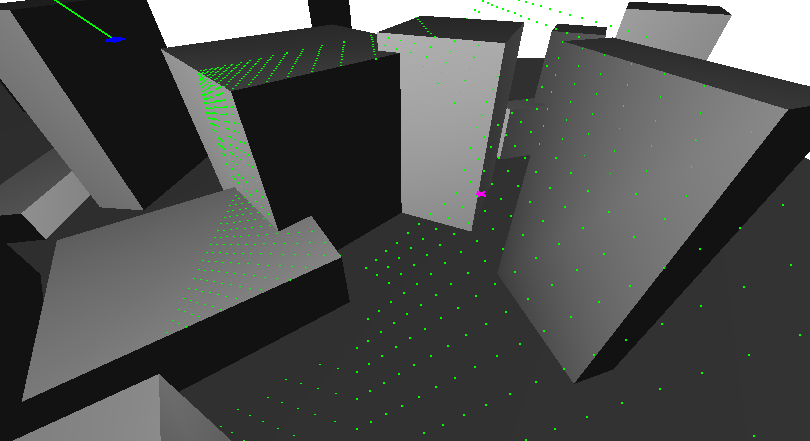
\includegraphics[width=\linewidth]{simDepthMap2.png}

    \vspace{5mm}
    
\includegraphics[width=\linewidth]{depthView.png}
    \vspace{-2.5cm}
    \end{wrapfigure}

    1. Получаем карту глубин

    2. С помощью обратной матрицы перспективной трансформации
    переводим каждую точку на карте глубин в точку в пространстве

$$
\vec U = \left( \begin{array}{c c c c}
        \frac{1}{ R \cdot \tan( \frac{1}{2} A ) } & 0 & 0 & 0 \\
        0 & \frac{1}{ \tan( \frac{1}{2} A ) } & 0 & 0 \\
        0 & 0 & \frac{ z_{n} + z_{f} }{ z_{n}-z_{f} } & \frac{ 2 \cdot z_{n} \cdot z_{f} }{ z_{n} - z_{f} } \\
        0 & 0 & -1 & 0 \end{array} \right)^{-1} 
    \left( \begin{array}{c} x \\ y \\ depth \\ 1 \end{array} \right)
$$

$$\vec P = \frac{( X_U, Y_U, Z_U )^T}{ W_U } $$

    3. Кадждую полученную точку и координаты камеры юнита
    приводим к системе координат карты и строим отрезок

    \begin{center}
    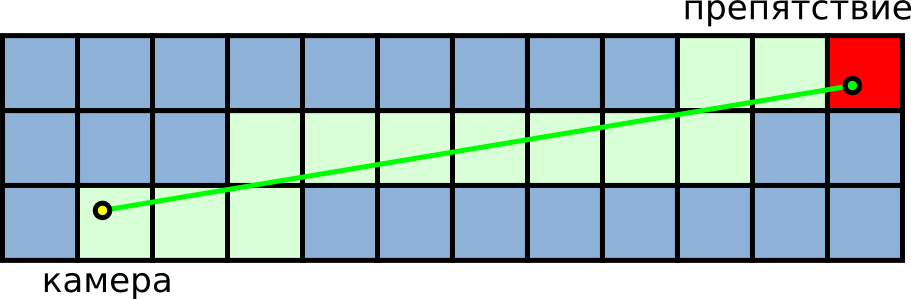
\includegraphics[width=.45\linewidth]{mapRaster.png}
    \end{center}

\end{tslide}

\begin{tslide}{Алгоритмы обхода местности}

    Было разработано 3 варианта алгоритма:

    \begin{tabular}{c c}
    \begin{tabular}{c}
    \begin{minipage}[h]{.4\linewidth}
    \begin{center}
    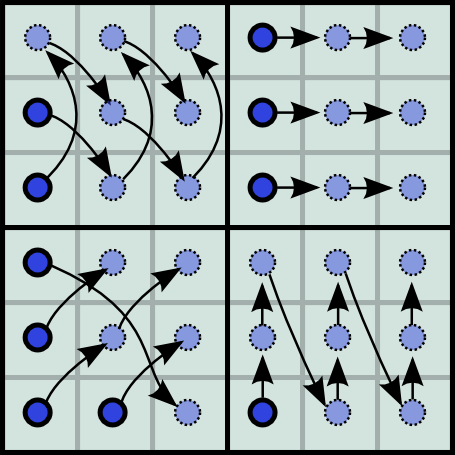
\includegraphics[width=6cm]{unitSerialMove.png}
    \linebreak
    \vspace{5mm} рис. 1 \vspace{5mm}
    \end{center}
    \end{minipage}
\\
    \begin{minipage}[h]{.4\linewidth}
    \begin{center}
    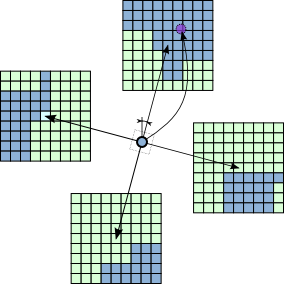
\includegraphics[width=6cm]{unitFineMove.png}
    \linebreak
    \vspace{5mm} рис. 2
    \end{center}
    \end{minipage}
    \end{tabular}
    &
    \begin{minipage}[h]{.5\linewidth}
    \begin{itemize}
    \item распределение подгрупп юнитов по регионам карты
            (рис. 1)
            \vspace{5mm}
    \item поиск ближайших неизведанных регионов
            (рис. 2)
            \vspace{5mm}
    \item выбор случайной точки в пределах карты
    \end{itemize}
    \end{minipage}
    \end{tabular}

\end{tslide}

\begin{tslide}{Момент смены целевой точки}

    \tikzstyle{startnode} = [circle,minimum size=.5cm,fill=black]
    \tikzstyle{stepnode} = [draw,rectangle, minimum height=0.7cm,
                text centered, rounded corners]
    \tikzstyle{endnode} = [circle,minimum size=.5cm,fill=white,draw=black]
    \tikzstyle{statnode} = [diamond,aspect=3,draw,text badly centered,inner sep=0pt]

    \begin{wrapfigure}{r}{0.3\linewidth}
    \begin{tikzpicture}[>=triangle 45,shorten >= 0pt,auto,node distance=2cm]

        \node[startnode] (0) {};
        \node[stepnode] (1) [below of=0] {\verb|n++|};
        \node[statnode] (2) [below of=1] {\verb|n >= K|};
        \node[endnode] (r1) [right=2cm of 2] {};
        \node[statnode] (3) [below of=2] {\verb|D < limit|};
        \node[endnode] (r2) [below of=r1] {};
        \node[stepnode] (4) [below of=3] {\verb|n=0|};
        \node[stepnode] (5) [below of=4] {\verb|choiseTarget()|};
        \node[endnode] (6) [below of=5] {};

        \path[->]
        (0) edge (1) 
        (1) edge (2) 
        (2) edge (3)
        (3) edge (4)
        (2) edge node[above] {$\text{нет}$} (r1)
        (3) edge node[above] {$\text{нет}$} (r2)
        (4) edge (5)
        (5) edge (6);

    \end{tikzpicture}

    \end{wrapfigure}

    \verb|n| -- счётчик шагов

    \verb|K| -- минимальное количество шагов, необходимое для смены целевой
                точки

    \verb|D| -- дисперсия расстояния до цели за последние \verb|K| шагов

    \verb|limit| -- порог для значения дисперсии

\end{tslide}

\begin{tslide}{Программно-математическое обеспечение}

    ПМО состоит из:
    \begin{itemize}
        \item Базовой части -- работа с векторами, матрицами, системы
    взаимодействия классов, управление внешней для GC памятью

        \item Графической части -- оконная система, классовые обёртки
            для работы с \verb|OpenGL|

        \item Симуляции МБПЛА -- модель юнита и вспомогательные
            классы для работы с ней, интерфейс модели карты

        \item Гетерогенных вычислений с использованием \verb|OpenCL| --
            их нельзя полностью отнести к симуляции МБПЛА, так как
            они тесно связанны с графической частью. К ним относится
            релализация карты и её отрисовка.
    \end{itemize}


\end{tslide}

\begin{tslide}{Программно-математическое обеспечение}

    \centering
    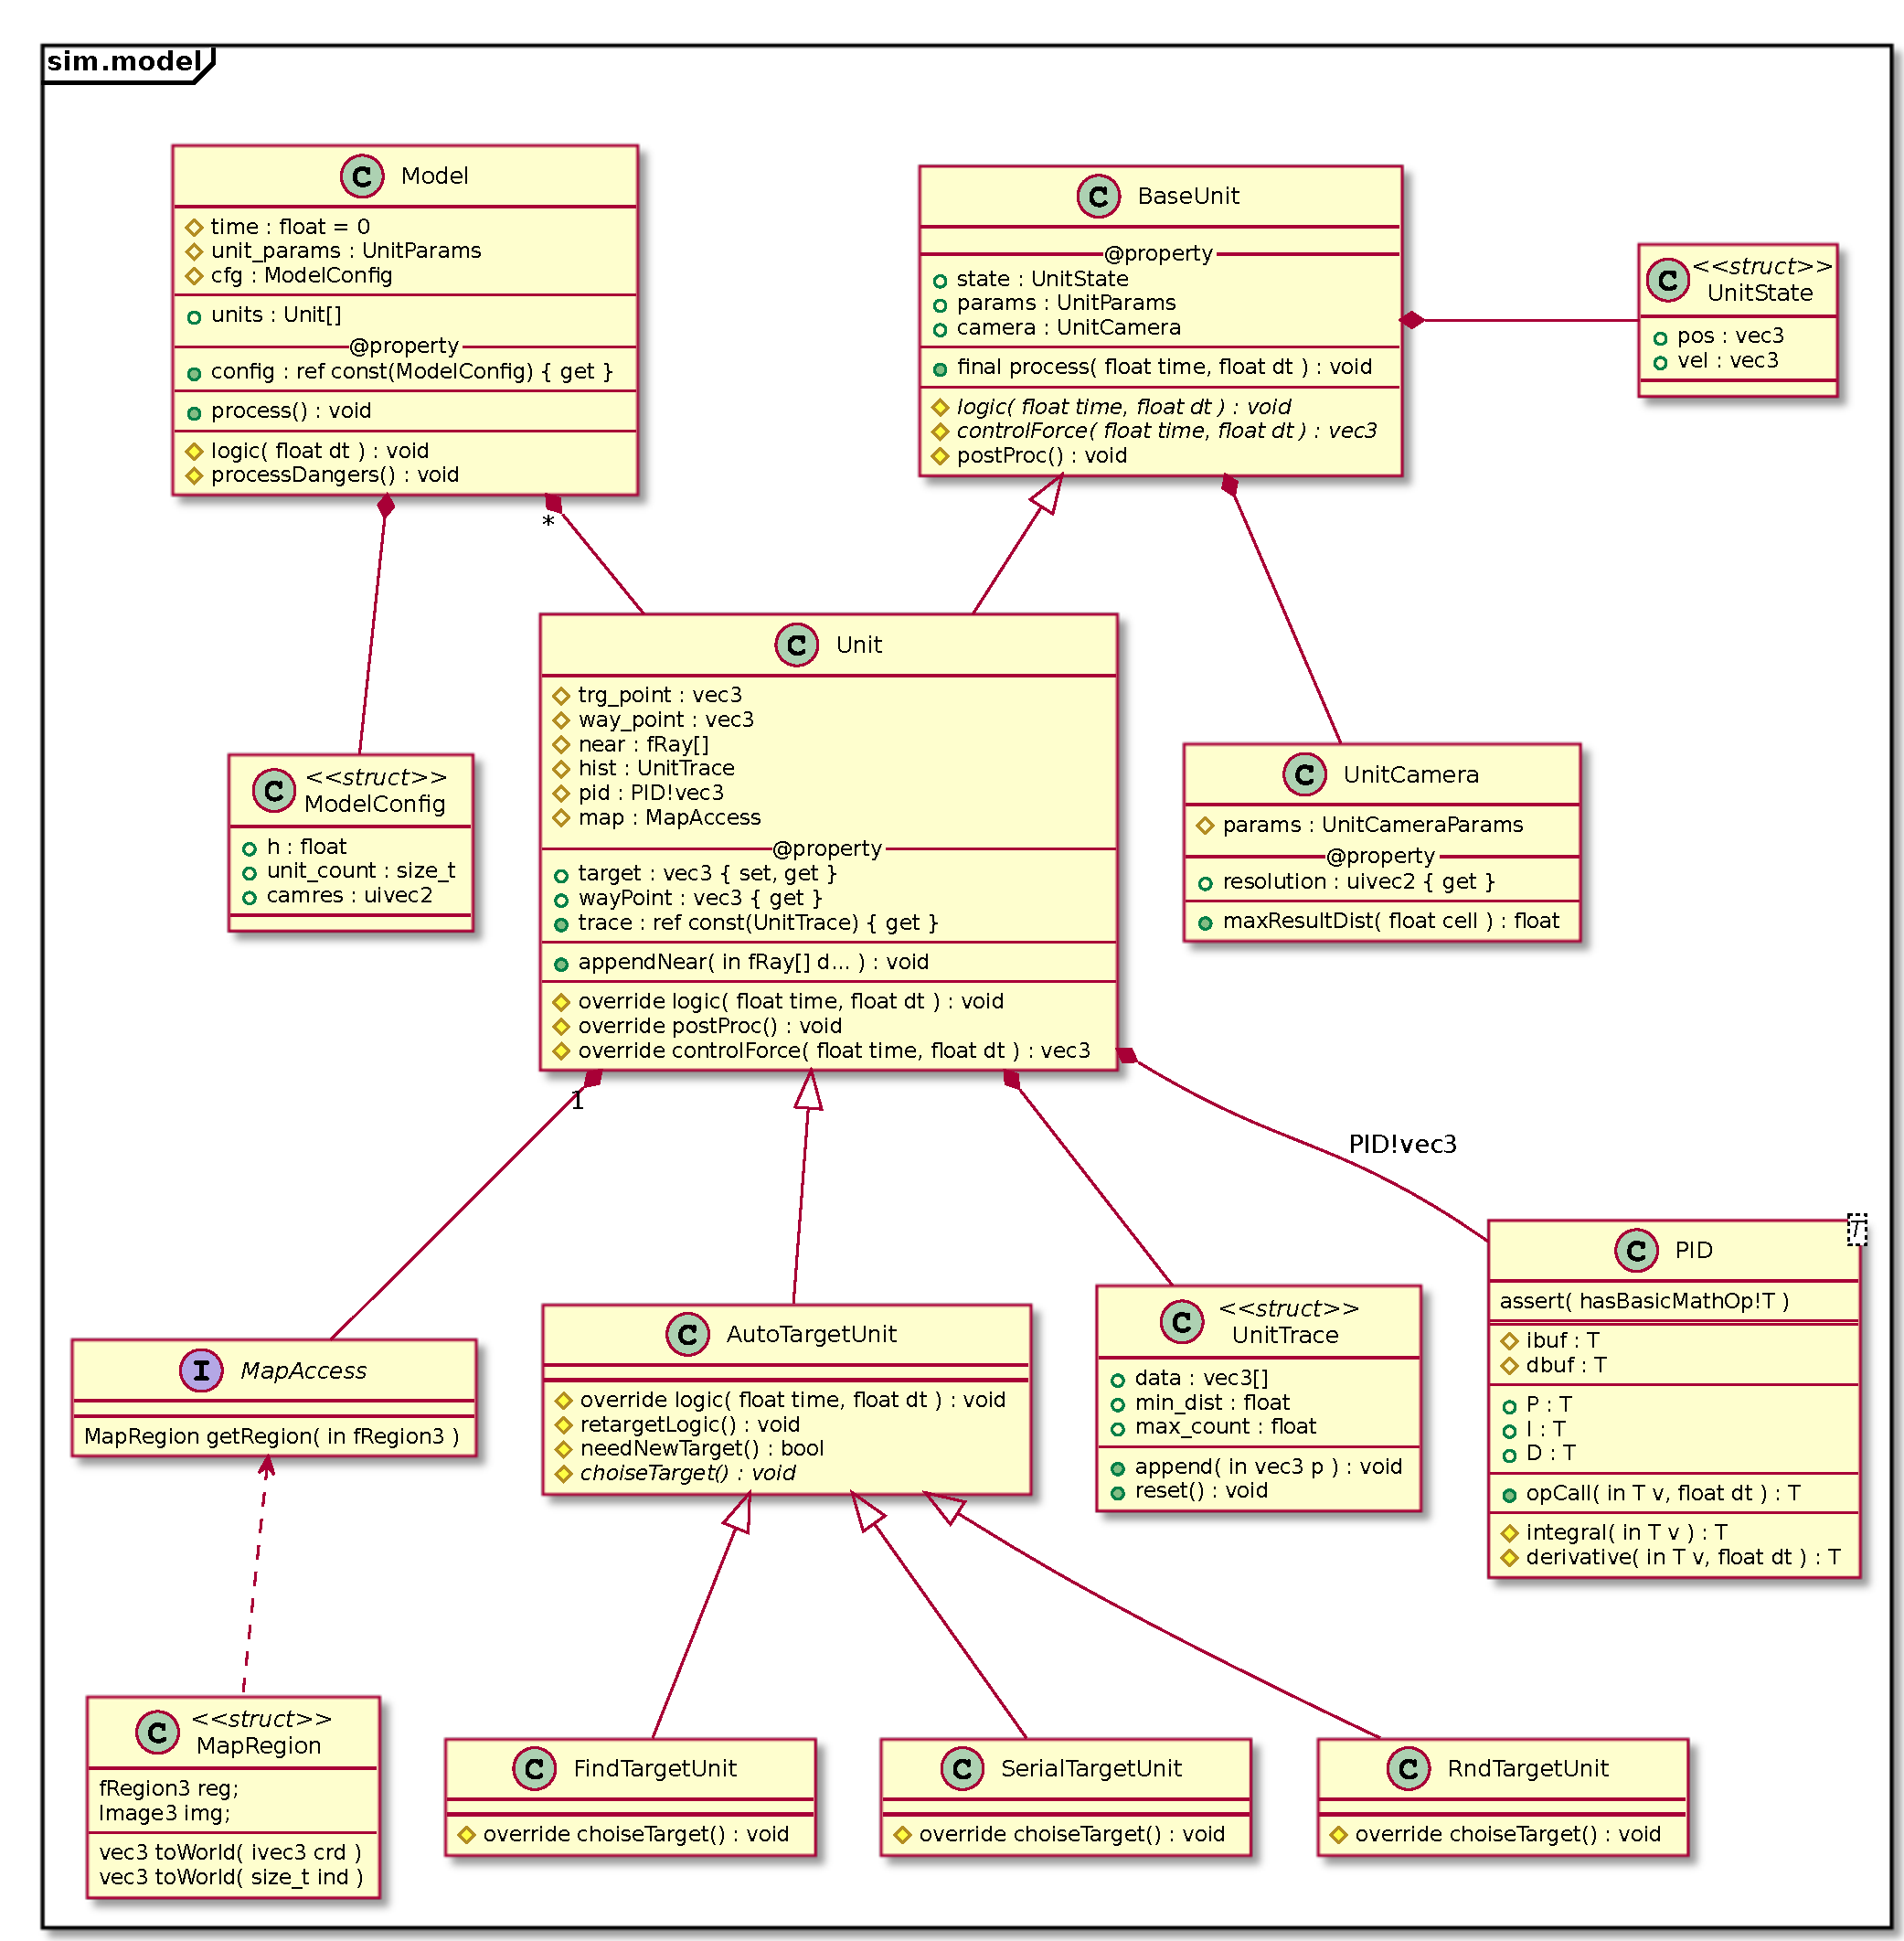
\includegraphics[width=.6\linewidth]{model_uml.eps}

    Диаграмма классов модуля симуляции МБПЛА
\end{tslide}

\begin{tslide}{Результаты экспериментов}
    \vfill
    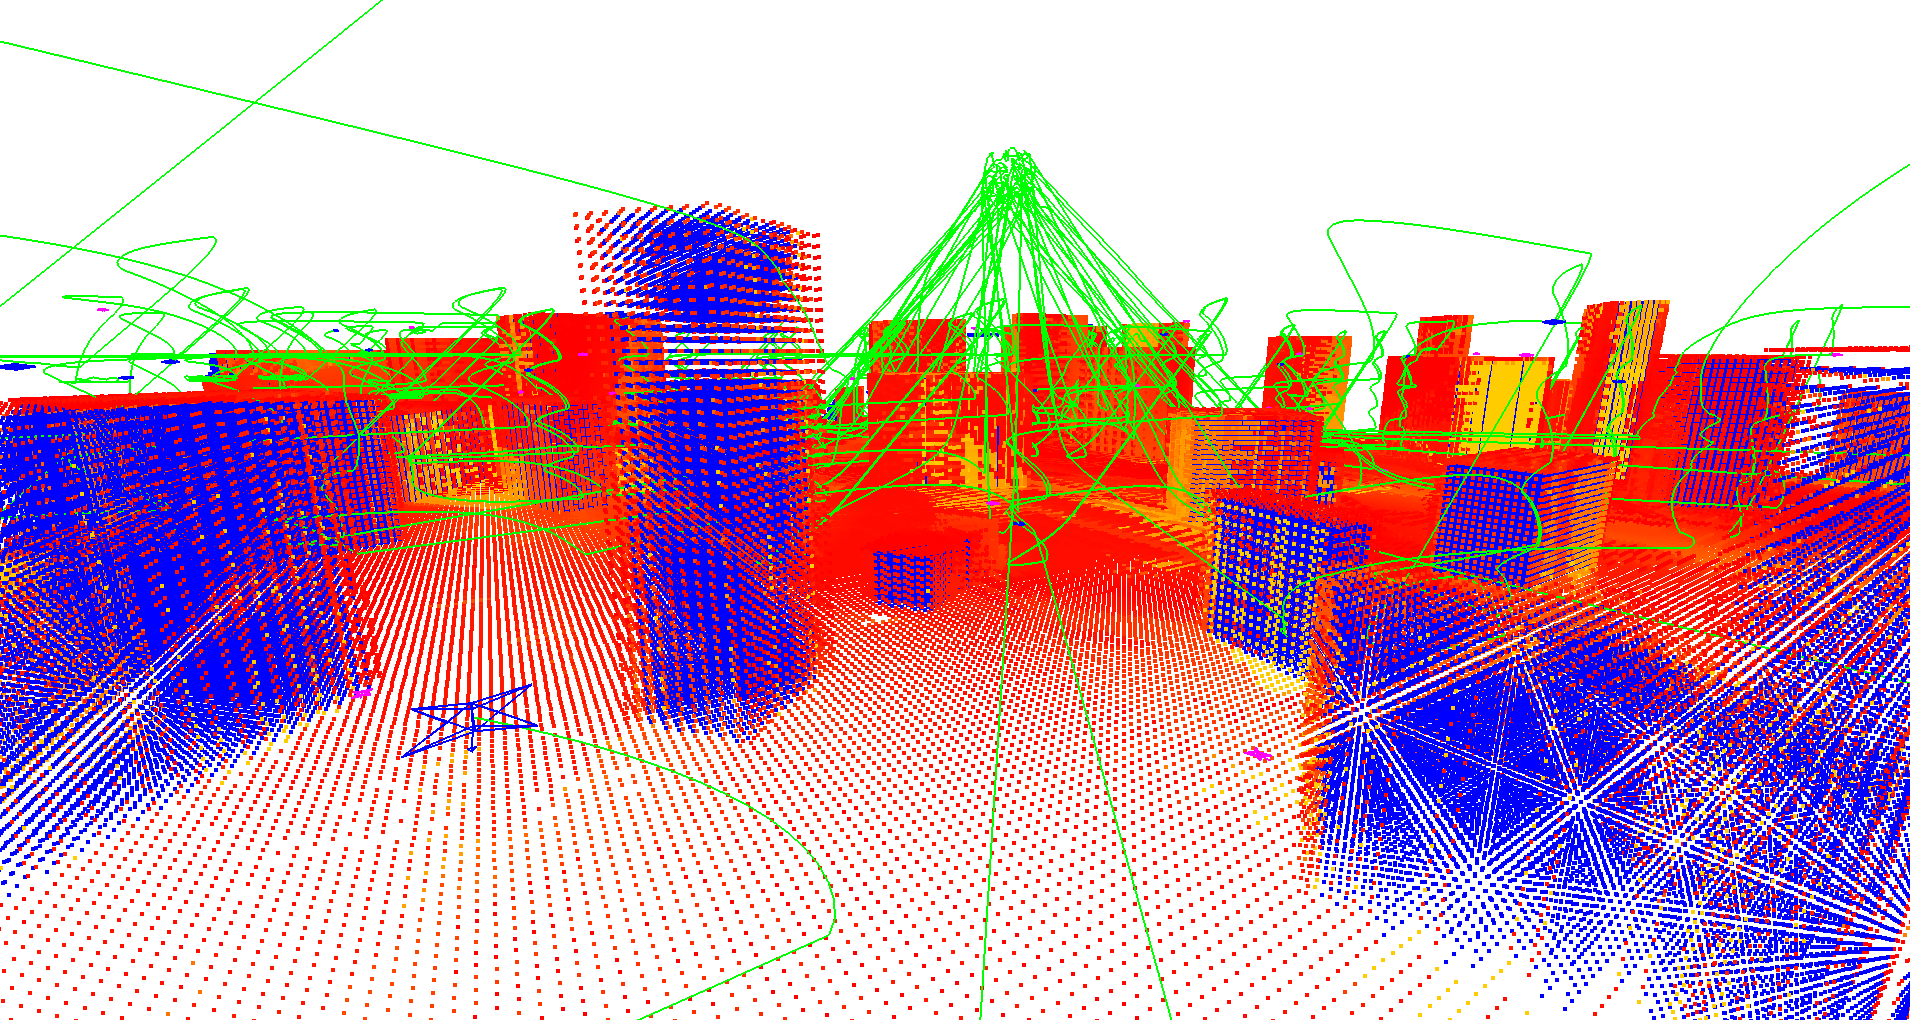
\includegraphics[width=\linewidth]{s50s_map2.png}
    \vfill
\end{tslide}

\begin{tslide}{Результаты работы МБПЛА с алгоритмом поиска ближайшего неизведанного региона}

    \vfill
    \centering
    \begin{tabular}{l r}
    \begin{minipage}[h]{.5\linewidth}
    \centering
    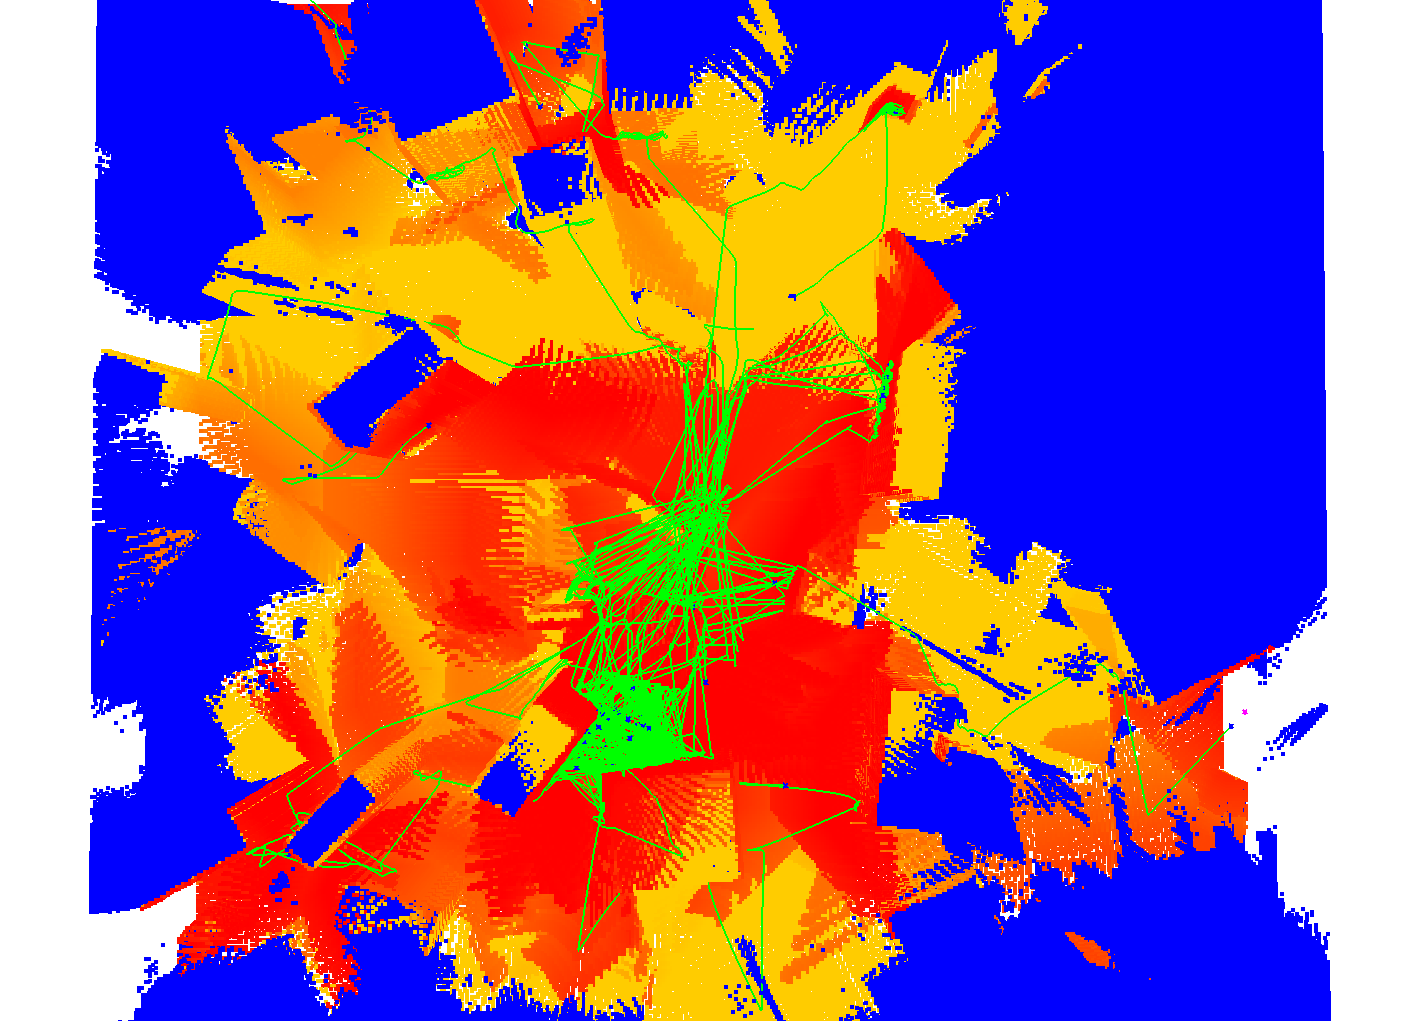
\includegraphics[width=\linewidth]{s50f4r_map.png}
    \end{minipage}
    &
    \begin{minipage}[h]{.5\linewidth}
    \centering
    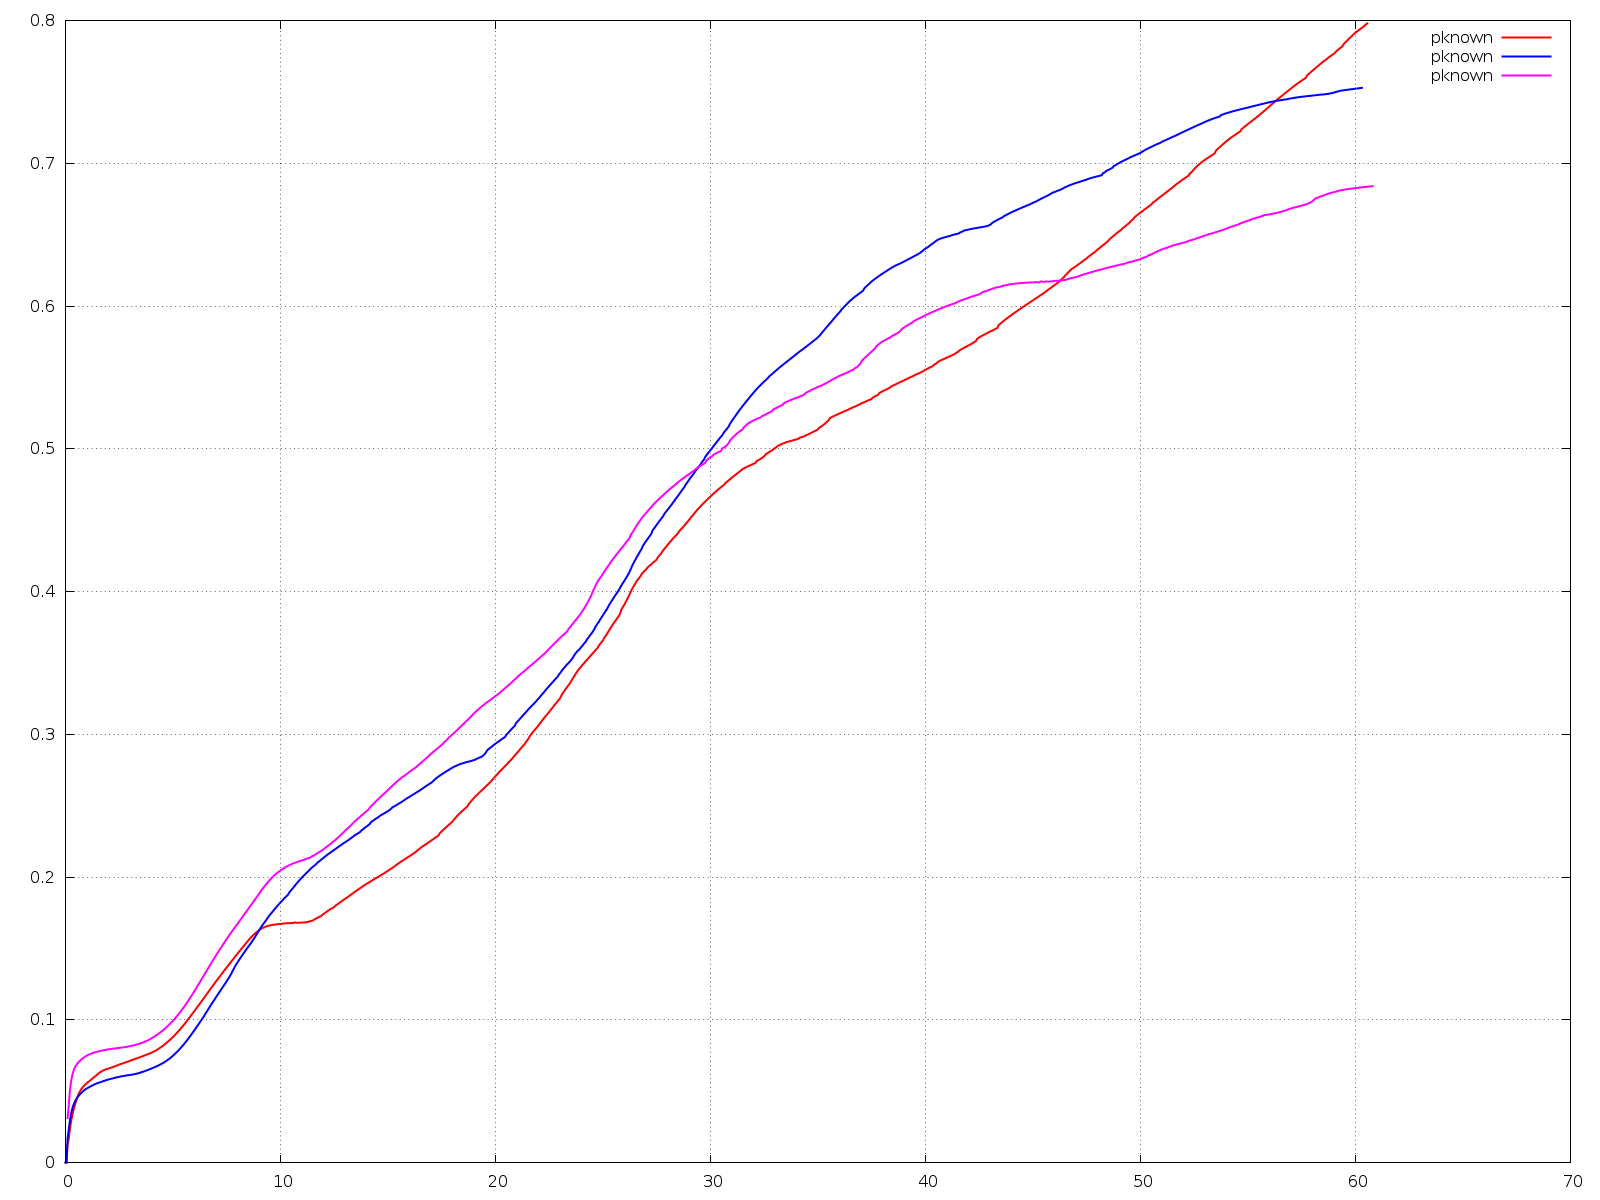
\includegraphics[width=.5\linewidth]{all_find_4_pknown.png}

    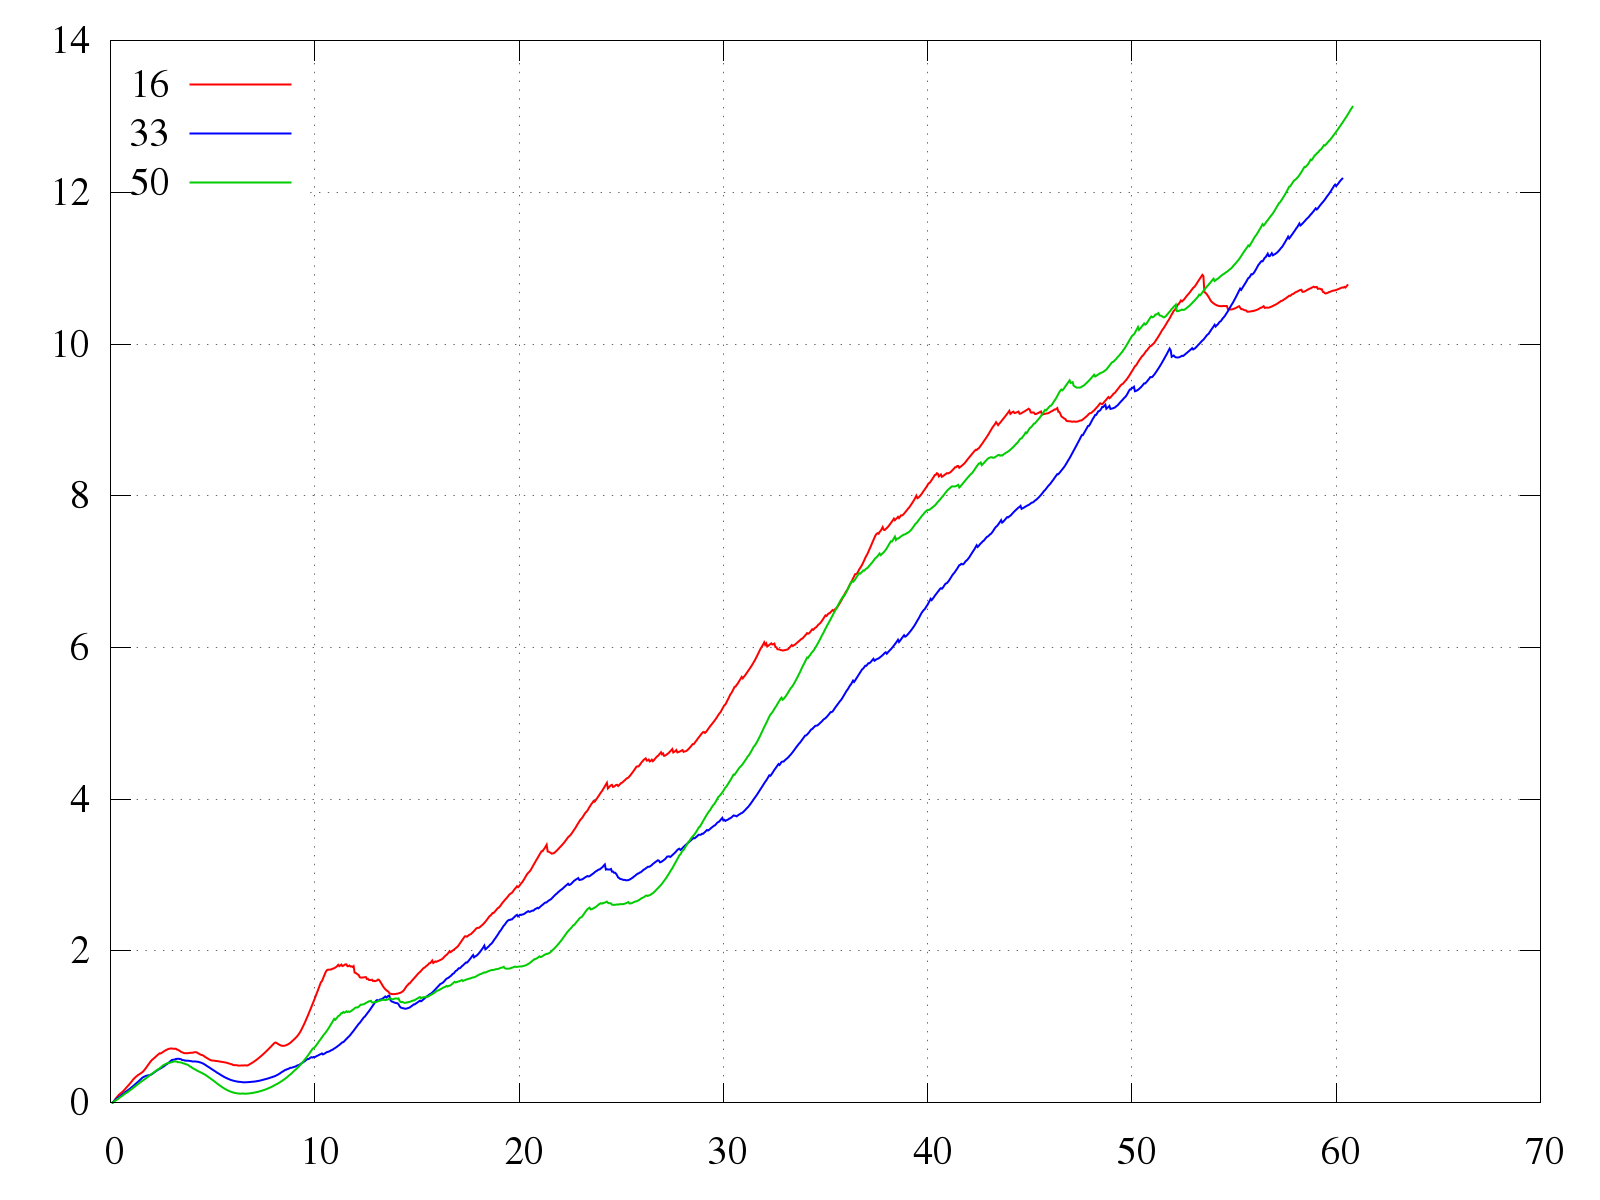
\includegraphics[width=.5\linewidth]{all_find_4_ts.png}
    \end{minipage}
    \end{tabular}
    \vfill

\end{tslide}

\begin{tslide}{Результаты работы МБПЛА со выставлением случайной точки к пределах карты}

    \vfill
    \centering
    \begin{tabular}{l r}
    \begin{minipage}[h]{.5\linewidth}
    \centering
    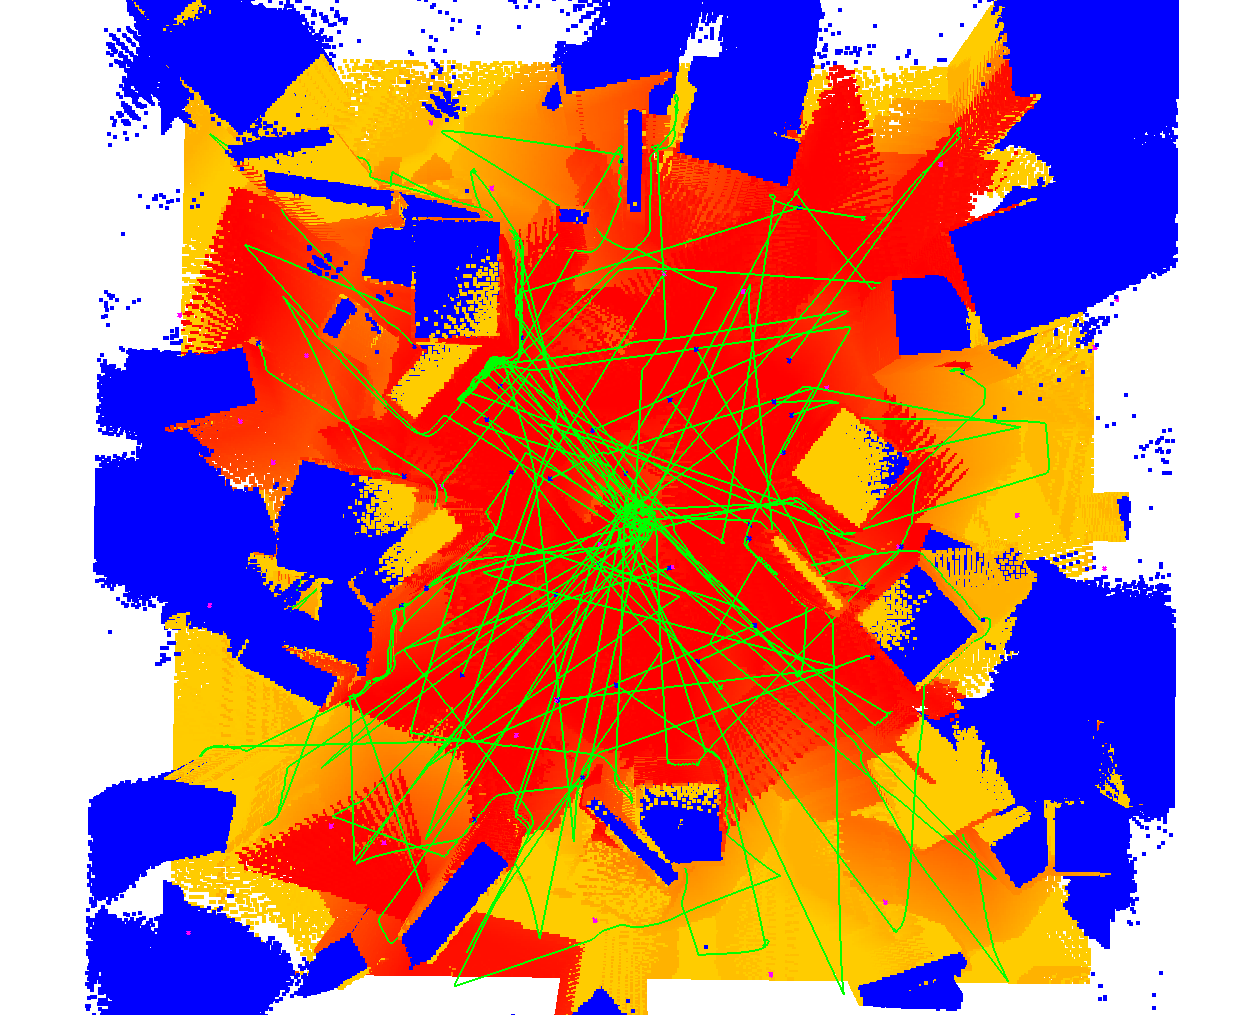
\includegraphics[width=\linewidth]{s50rm_map.png}
    \end{minipage}
    &
    \begin{minipage}[h]{.5\linewidth}
    \centering
    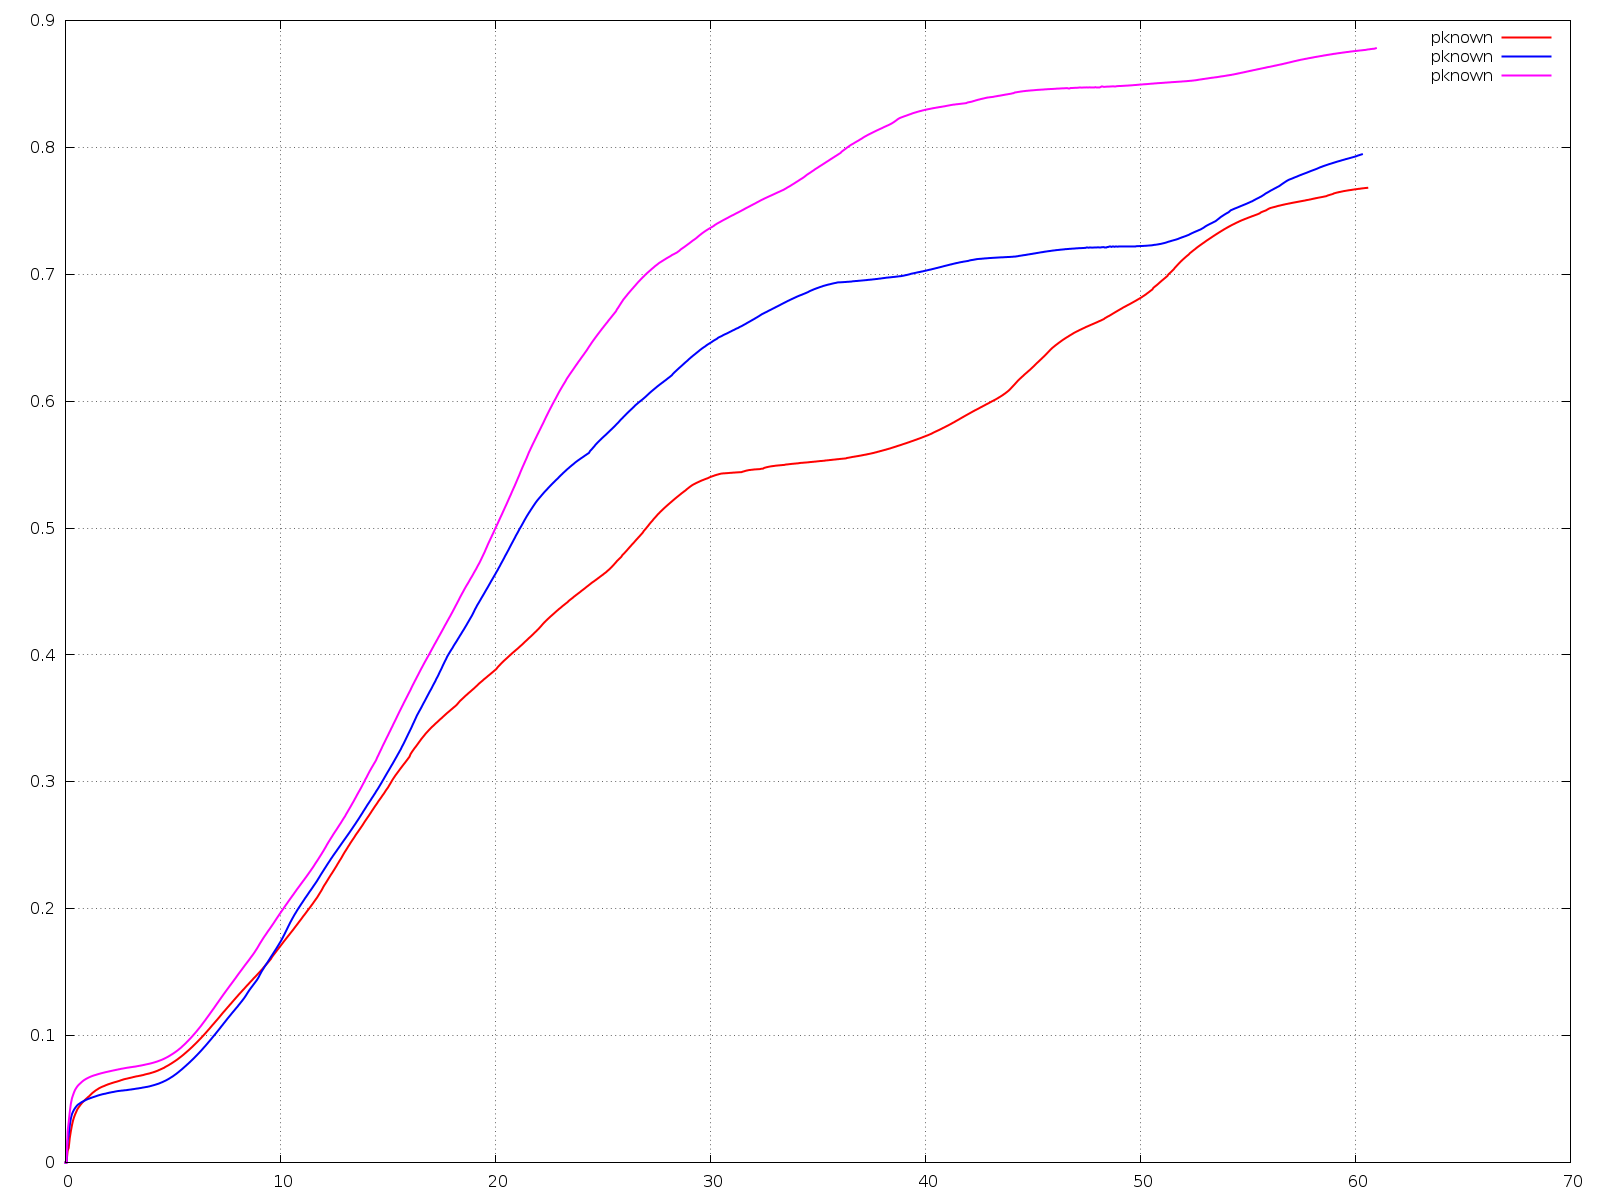
\includegraphics[width=.5\linewidth]{all_rnd_auto_pknown.png}

    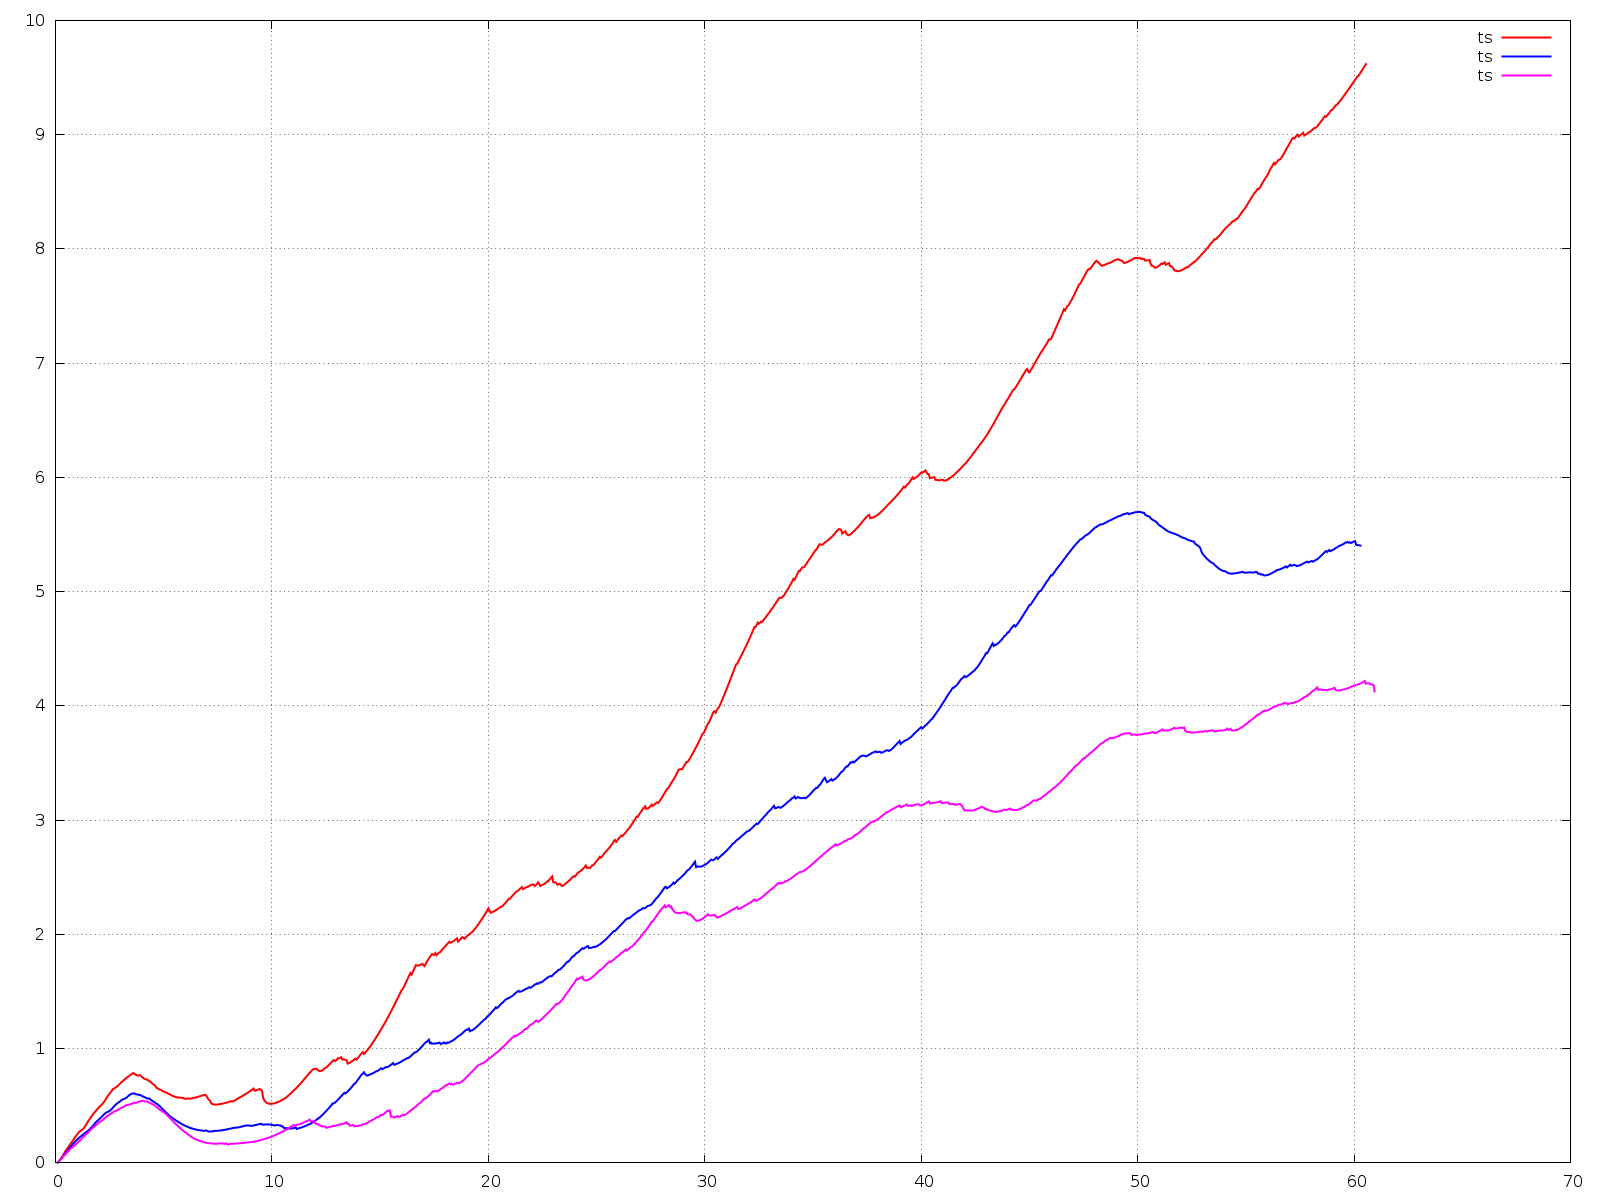
\includegraphics[width=.5\linewidth]{all_rnd_auto_ts.png}
    \end{minipage}
    \end{tabular}
    \vfill

\end{tslide}

\begin{tslide}{Результаты работы МБПЛА с алгоритмом распределения подгрупп по регионам}

    \vfill
    \centering
    \begin{tabular}{l r}
    \begin{minipage}[h]{.5\linewidth}
    \centering
    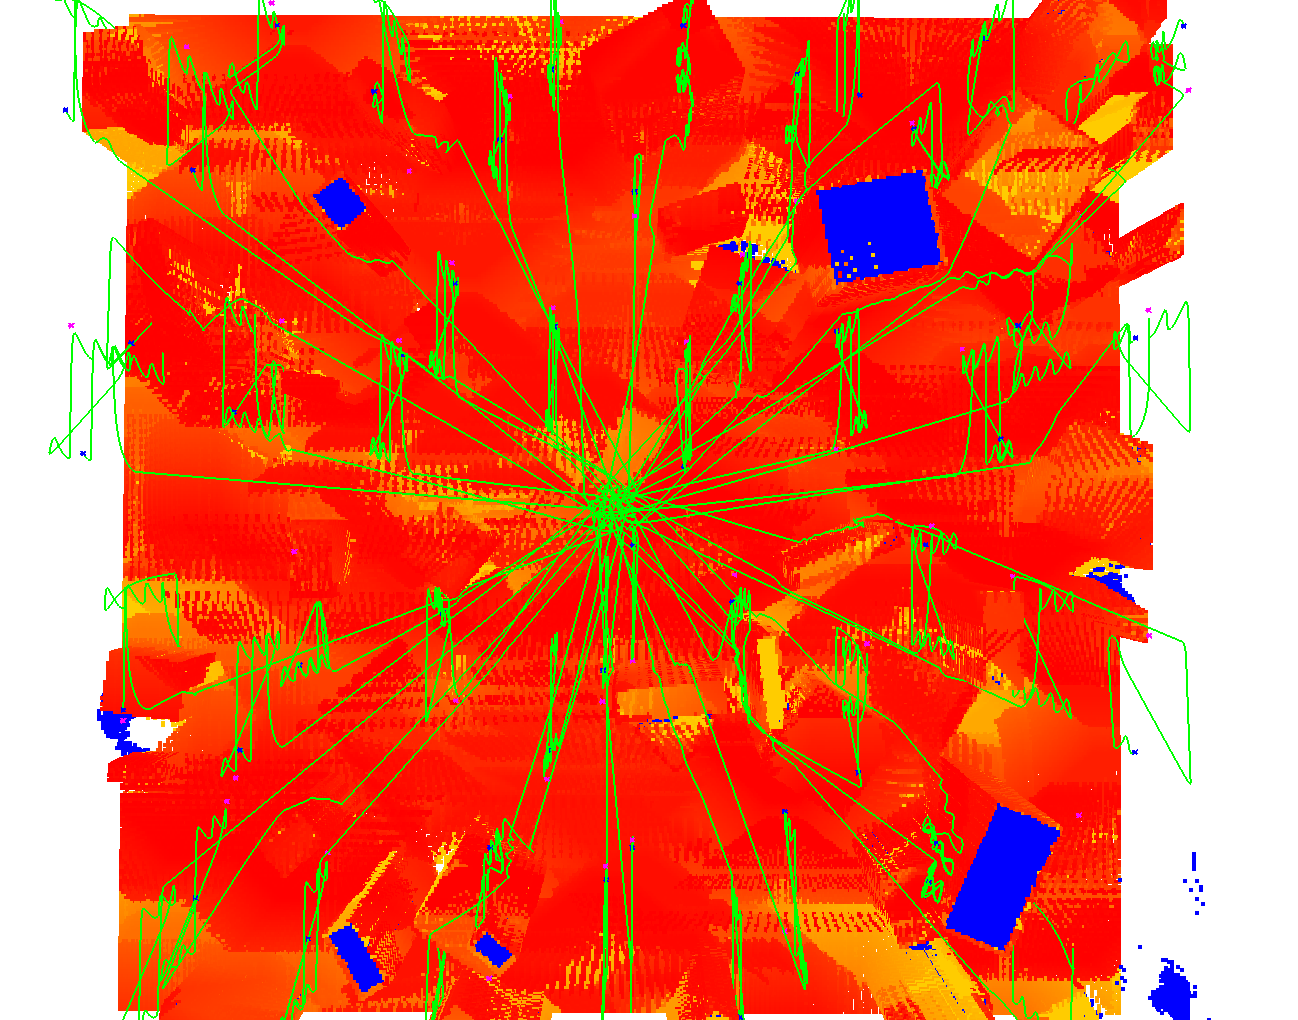
\includegraphics[width=\linewidth]{s50s_map1.png}
    \end{minipage}
    &
    \begin{minipage}[h]{.5\linewidth}
    \centering
    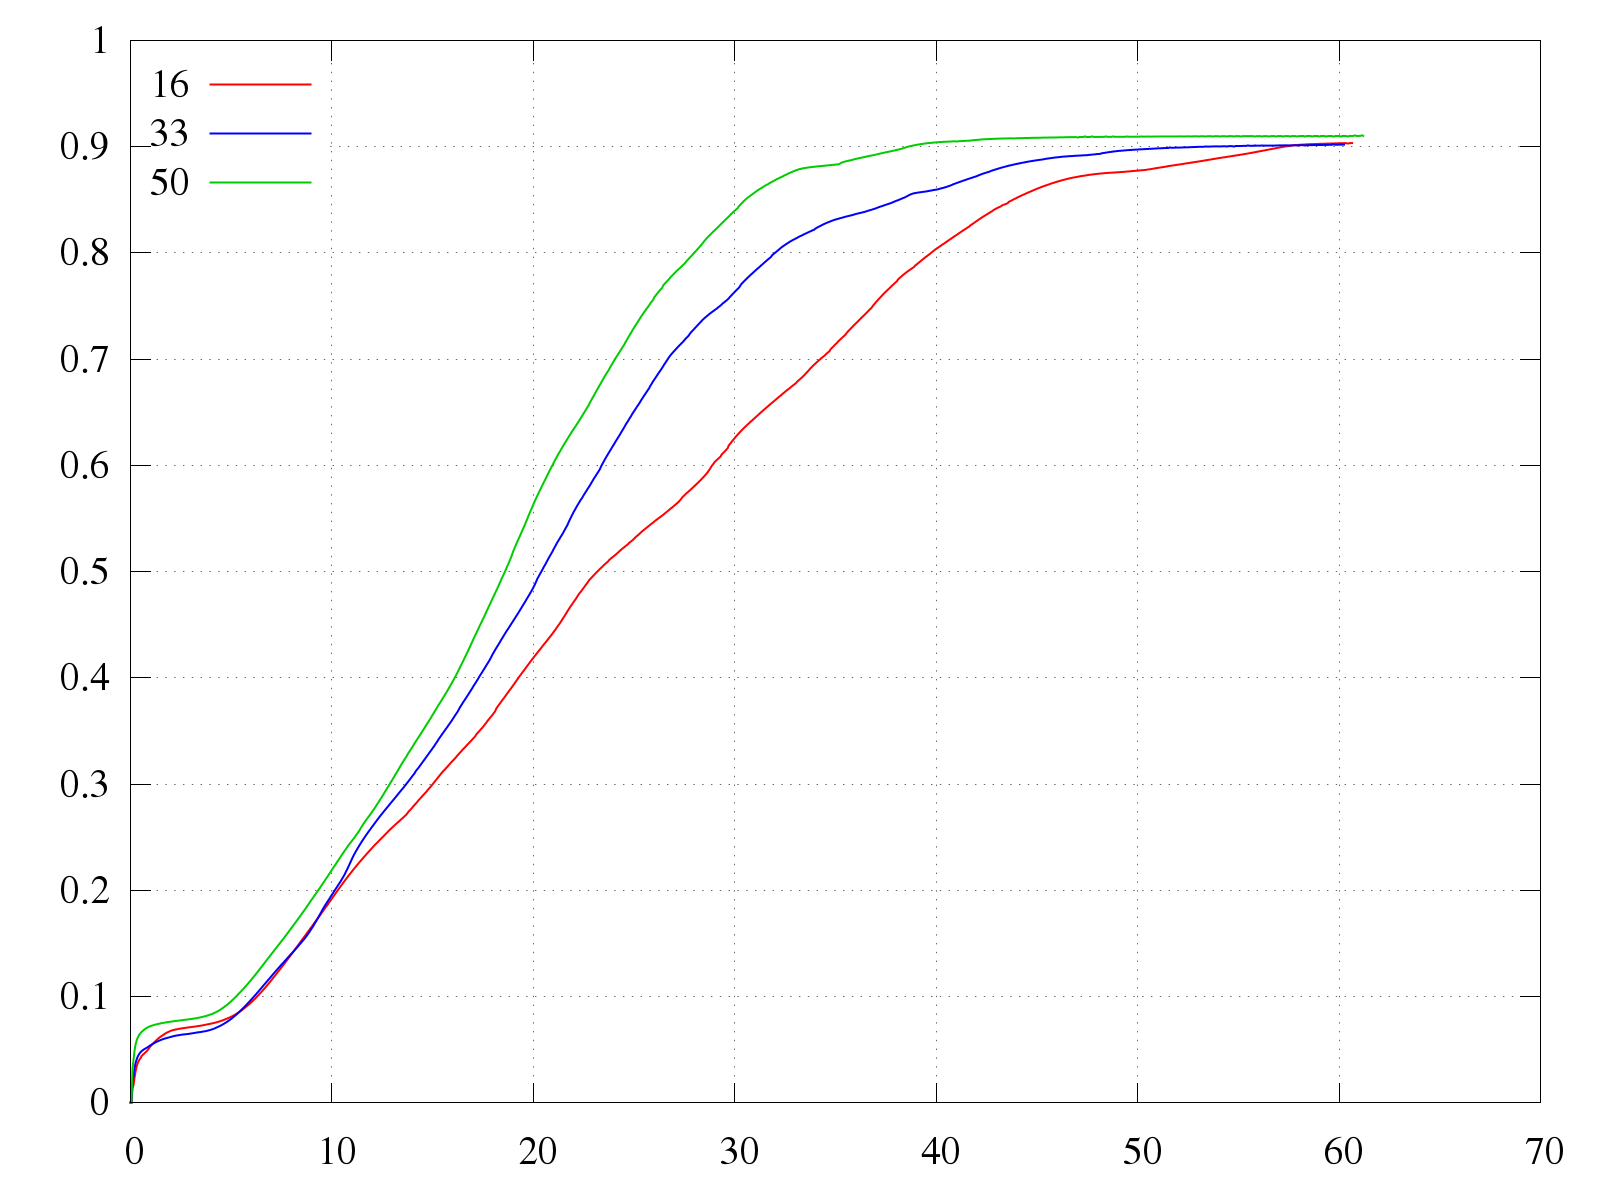
\includegraphics[width=.5\linewidth]{all_serial_pknown.png}

    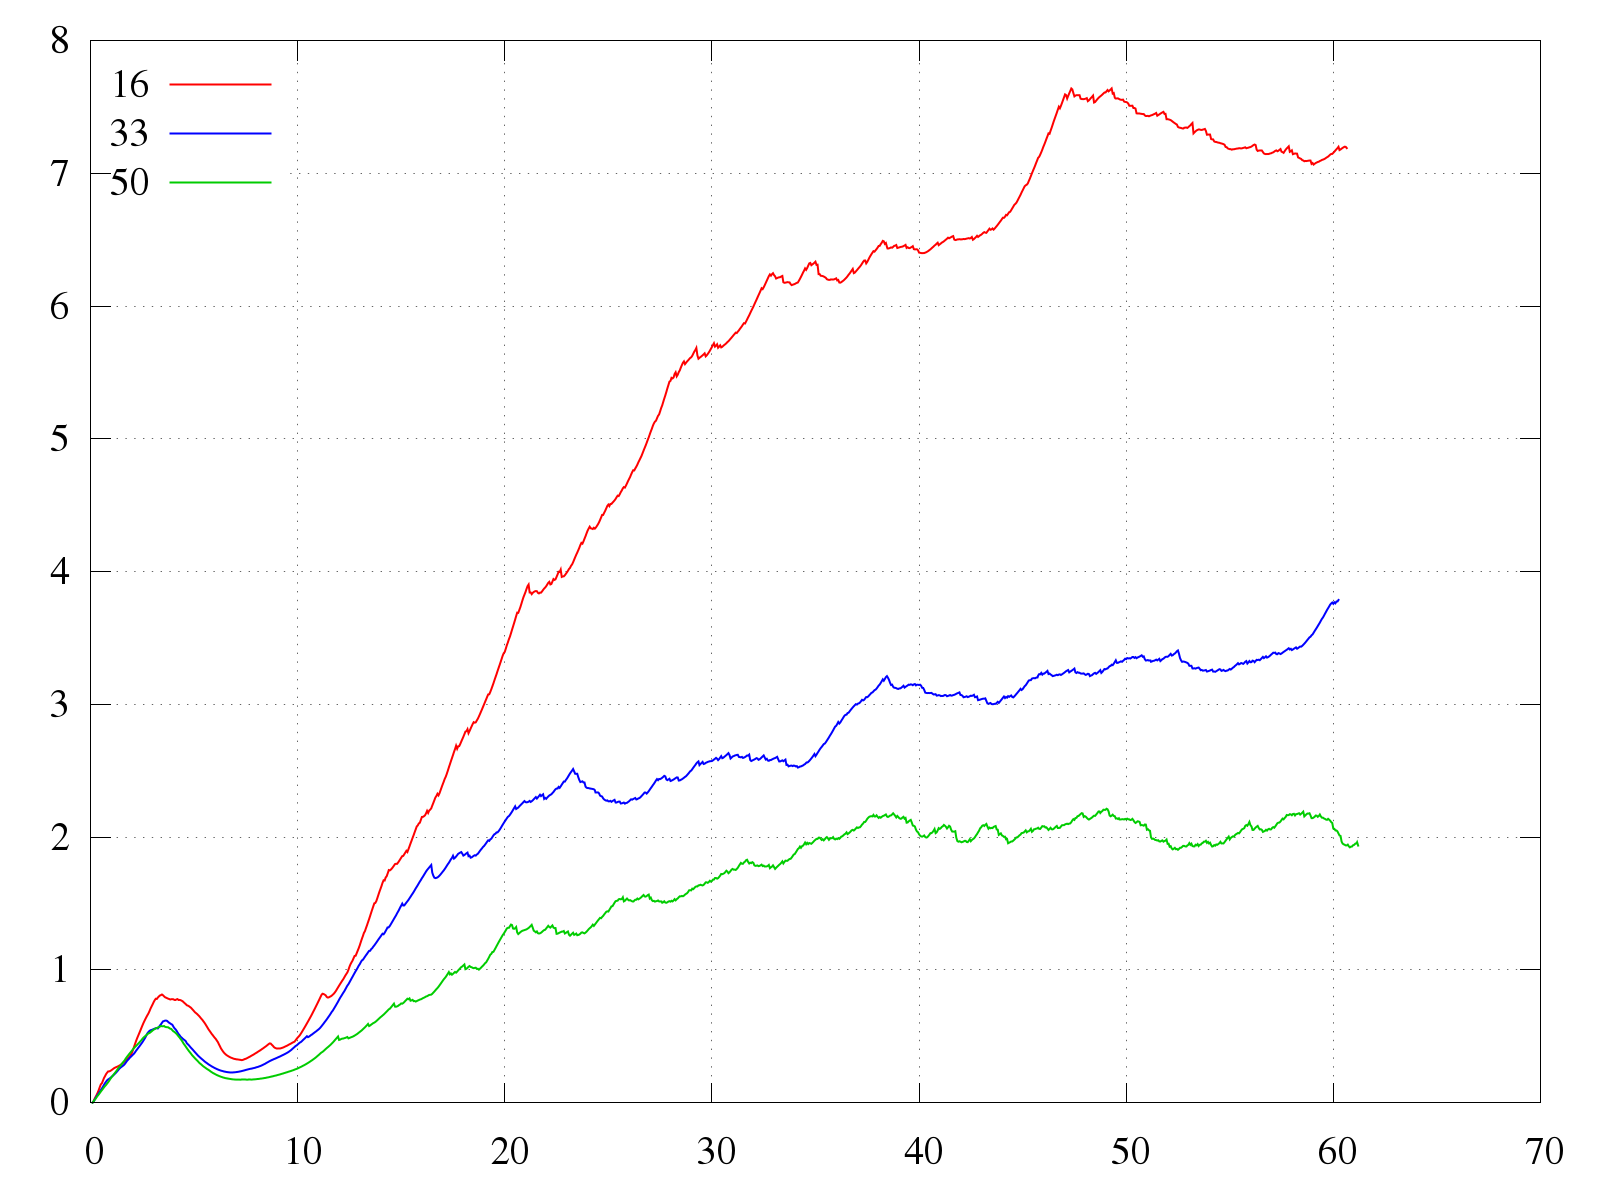
\includegraphics[width=.5\linewidth]{all_serial_ts.png}
    \end{minipage}
    \end{tabular}
    \vfill

\end{tslide}

\begin{tslide}{Сравнение работы алгоритмов}

    \centering
    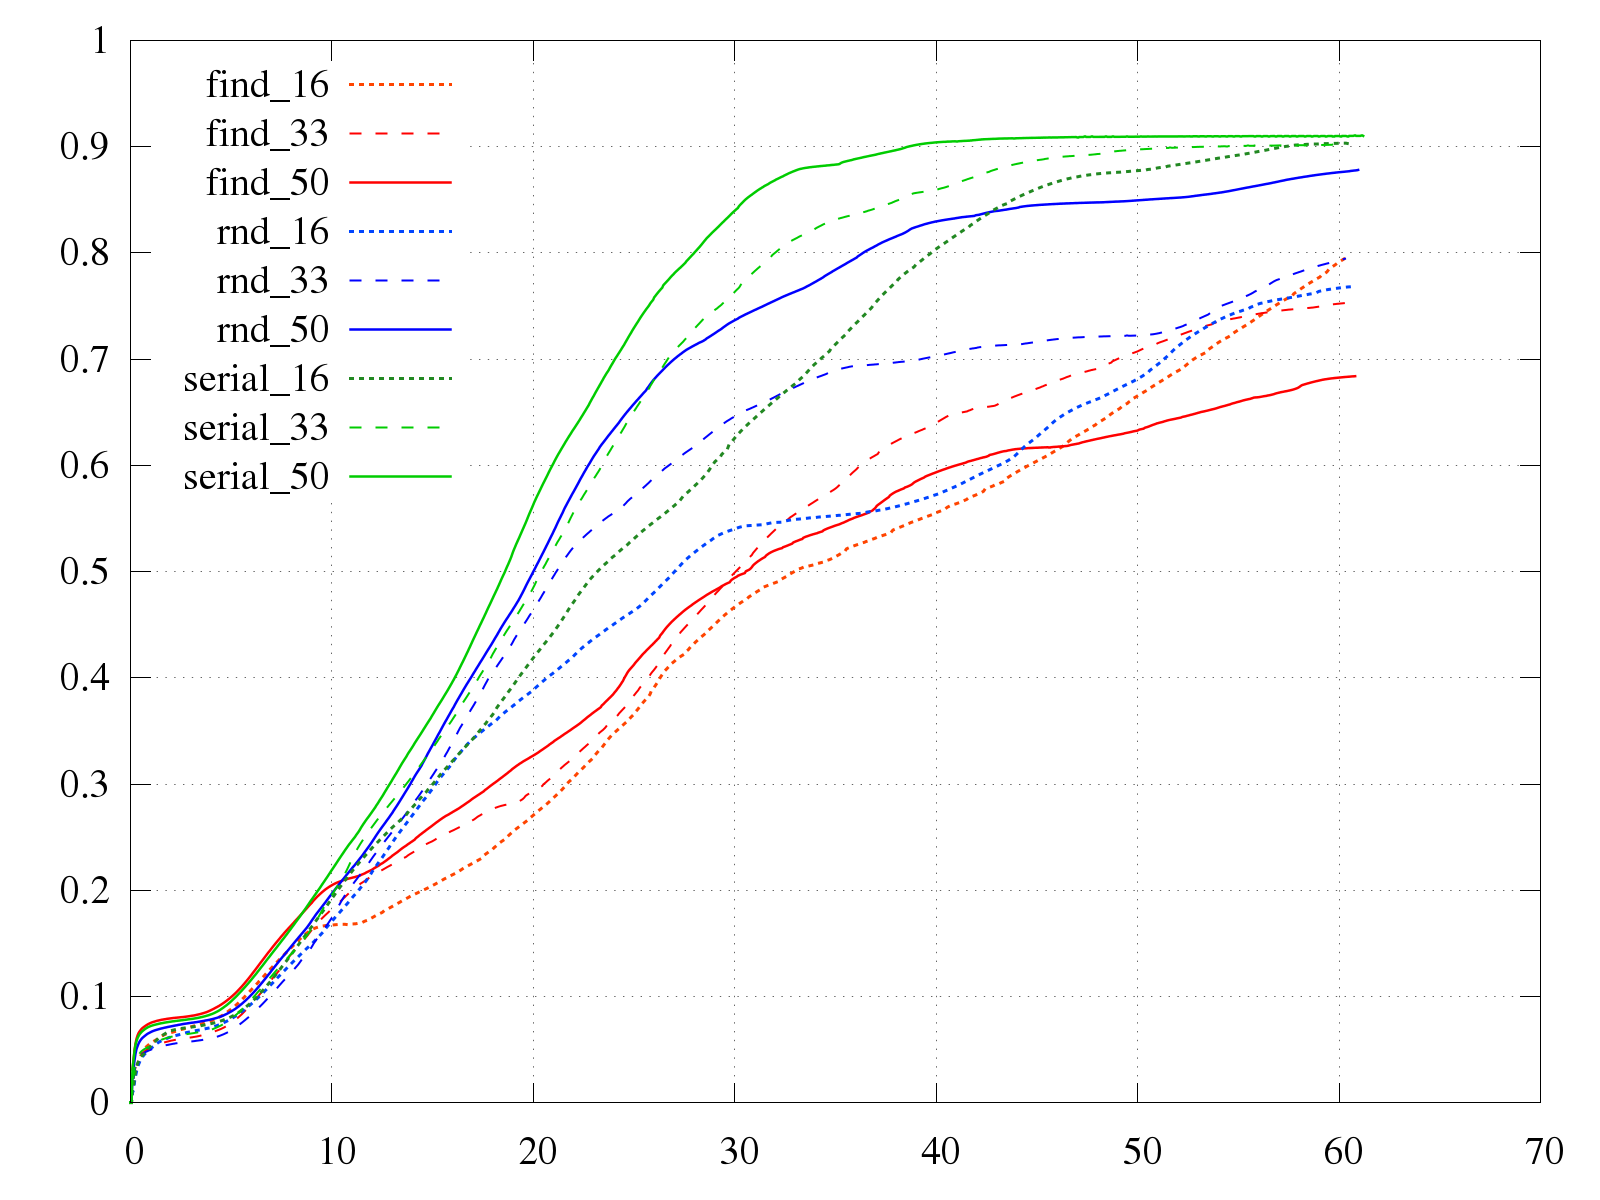
\includegraphics[width=.9\linewidth]{all_pknown.png}

\end{tslide}

\begin{tslide}{Сравнение работы алгоритмов}

    \centering
    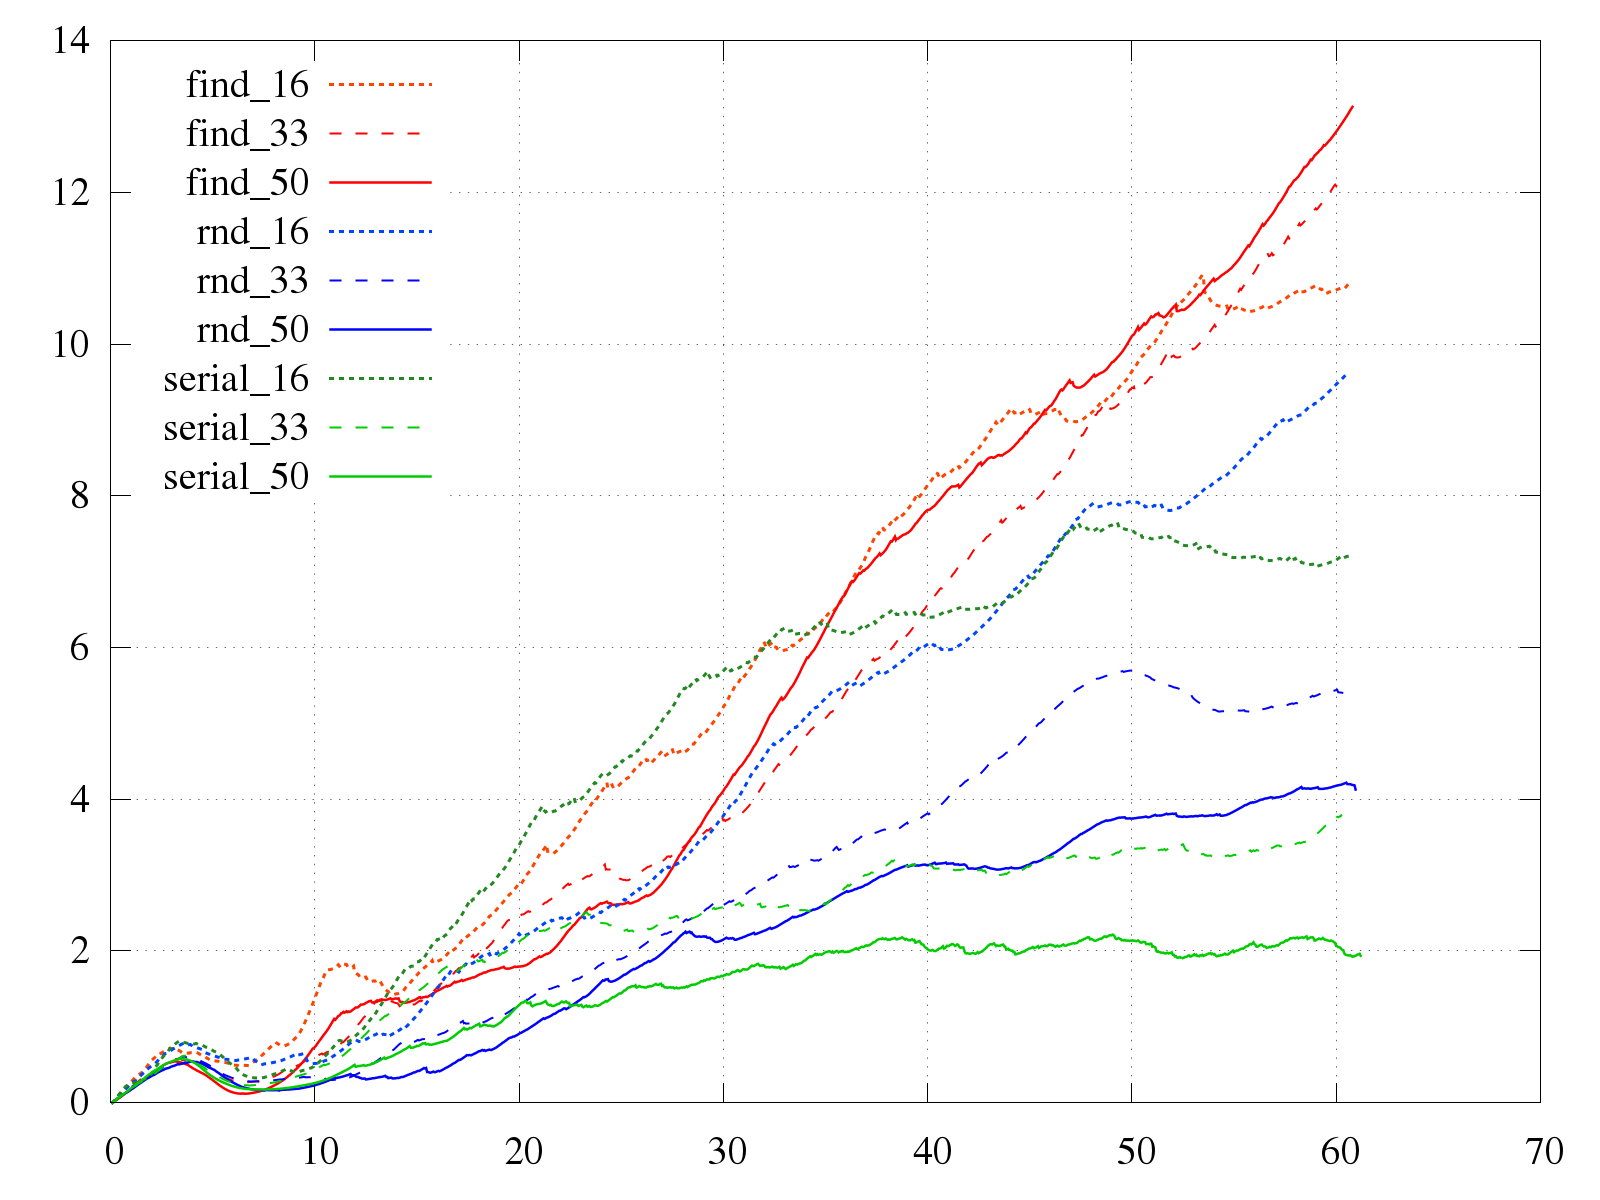
\includegraphics[width=.9\linewidth]{all_ts.png}

\end{tslide}

\begin{tslide}{Заключение}

    \begin{itemize}
    \item Разработан алгоритм построения 3х мерной карты местности 
        с использованием МБПЛА
    \item Реализовано программно-математическое обеспечение, с
        помощью которого было произведенно моделирование работы
        МБПЛА и получены результаты экспериментов, как графических
        так и численных.
    \item Проведён анализ результатов экспериментов, который показал
        наличие недостатков и достоинств каждого из вариантов
        алгоритма обхода местности. В итоге можно сказать, что
        чем равномернее распределены юниты по карте и чем меньше
        им необходимо перемещаться, тем лучше результат по 
        поддержанию актуальности карты.
    \end{itemize}

\end{tslide}

\begin{cslide}
    \LARGE Спасибо за внимание.
\end{cslide}

\end{document}
